\documentclass[12pt, twoside]{report}
%\documentclass[12pt]{report}		

%%% CHOOSE THE COLOR SCHEME %%%
% User defined color which will be used throughout the document
% In case you want another color, find its HTML code (without #), a 6-digit string consisting of numbers and letters, then replace it in the brackets
\def\htmlmaincolorcode{607B8B} 
% Analogously, choose the color for shaded equation boxes, in case you wish to use them
\def\htmlshadecolorcode{E4EDF2}
% If you don't want any color and prefer black, just replace the option [customcolor] with [black]
\usepackage[customcolor]{ctp-fpub}

\usepackage{biblatex}
\bibliography{references}


%%% ADD HERE ALL THE PACKAGES YOU USE %%%
% Packages required only for the specific content in this template, remove if not needed
\usepackage{slashed}
\usepackage{dsfont}
\usepackage{amsmath}
\usepackage{amssymb}
\usepackage{bm}
\usepackage{verbatim}


%%% COMMANDS & PACKAGES FOR TIKZIT %%%
%%% Requires tikzit.sty in the main folder, remove if not needed
\usepackage{tikzit}
\definecolor{gaugelink}{HTML}{87608b}
\definecolor{plaquette}{HTML}{607b8b}
\input{tikzit/plaquettes.tikzstyles}
% Package needed to scale .tikz diagrams
\usepackage{tikzscale}
\usepackage{multirow}
\usepackage{caption}
\captionsetup[figure]{font=footnotesize}

\usepackage{subcaption}
\captionsetup{compatibility=false}

\usepackage[toc,page]{appendix}
\usepackage{listings}

% If you want to compile just a part of the thesis use \includeonly
% For example:
% \includeonly{filename2,filename3}


%%% REPLACE THE INFORMATION IN THE BRACKETS %%%
% Information contained in the title page
\def\studentname{Gabriel Tiberiu Pan\u{a}} 
\def\thesistitle{Properties of \\seismic scale-free networks}
% In case of no subtitle, just leave this field empty {}
\def\thesissubtitle{applications for Romania, United States of America, Italy and Japan}
\def\thesistype{Master}
\def\firstsupervisor{Alexandru Nicolin}
\def\firstsupervisorprefix{Conf. Univ. Dr.}
% In case of no second supervsior, just leave these fields empty {}
\def\secondsupervisor{Virgil B\u{a}ran}
\def\secondsupervisorprefix{Prof. Univ. Dr.}
% In case of a third supervisor, well... 
\def\domeniu{Fizic\u{a} Teoretic\u{a} \c{s}i Computa\c{t}ional\u{a} / Theoretical and Computational Physics}
\def\tipteza{Master}

\begin{document}

% Title page
\newgeometry{margin=1in}
\newcommand{\itermediatevspace}{\vspace{0.15\textheight}}
\newcommand{\rowskip}{\vspace{\baselineskip}}
\newcommand{\tinyvspace}{\vspace{0.01\textheight}}
\newcommand{\mediumvspace}{\vspace{0.1\textheight}}
\newcommand{\bigvspace}{\vspace{0.2\textheight}}
\newcommand{\smallvspace}{\vspace{0.05\textheight}}
\newcommand{\topdoublerule}{
	\makebox[0pt][l]{\textcolor{\accentcolor}{\rule[4pt]{\linewidth}{1pt}}}%
    \rule[0pt]{\linewidth}{2pt}
}
\newcommand{\bottomdoublerule}{
	\makebox[0pt][l]{\rule[11pt]{\linewidth}{2pt}}%
    \textcolor{\accentcolor}{\rule[8pt]{\linewidth}{1pt}}
}

\begin{titlepage}

	\centering

	\begin{minipage}[c]{0.15\textwidth}
		\centering
		\includegraphics[height=0.1\textheight]{images/logo_university.png}
	\end{minipage}
	\begin{minipage}[c]{0.6\textwidth}
		\centering
		{\Large\scshape Universitatea din București}
		{\large Facultatea de Fizică}
	\end{minipage}
	\begin{minipage}[c]{0.15\textwidth}
		\centering
		\includegraphics[height=0.1\textheight]{images/logo_faculty.jpg}
	\end{minipage}

	\smallvspace
	
		{\Large\sffamily \studentname}
		
	\smallvspace
	
	\topdoublerule 
	\begin{spacing}{2.5}
		{\huge\scshape\sffamily \thesistitle}
		\ifthenelse{\equal{\thesissubtitle}{}}{
		}{
		\\ 
		{\large \thesissubtitle}
		}		
	\end{spacing}
	\bottomdoublerule
	
	\smallvspace
	
		{\large\scshape \thesistype\,Thesis}	
		
	\mediumvspace

	\begin{minipage}{\textwidth}
		\begin{flushright} \large
			{Scientific Advisers} \\[5pt]
			\firstsupervisorprefix\hspace{5pt}{\sffamily \firstsupervisor}\ifthenelse{\equal{\secondsupervisor}{}}{\rowskip}{\\\secondsupervisorprefix\hspace{5pt}{\sffamily \secondsupervisor}}			
		\end{flushright}
	\end{minipage}

	\ifthenelse{\equal{\thesissubtitle}{}}{\bigvspace}{\itermediatevspace}

	{\large Bucureşti, \the\year}
	
	

\end{titlepage}

\restoregeometry

{\pagestyle{empty}\cleardoublepage}


\tableofcontents
{\pagestyle{empty}\cleardoublepage}
\addtocontents{toc}{\protect\thispagestyle{empty}}

\pagenumbering{arabic}

% Don't include the .tex extension for the file name with include.
\addcontentsline{toc}{chapter}{Introduction}
\chapter*{Introduction}

In this work we wish to analyze various seismic regions around the globe from the perspective of complex networks. We expect that this would help give some insight into the mechanism of large events creation, avalanches of aftershocks and spatio-temporal span of these events and it would help us prove that earthquakes behave as a complex, self-organized critical system.\par 
This report is organized in five chapters: \par 
Chapter \ref{chap:complexSystems} is dedicated to familiarizing with terms such as complex systems, critical systems, self-organization and self-organization to criticality. A short history and introduction in network theory and graph theory is also presented. \par 
Chapter \ref{chap:quakeModels} deals with the most known system that shows self-organization to criticality behaviour, the classical sandpile model. The simplified and the original model help us understand this peculiar characteristic that appears in some complex systems in nature. Also, a staple model of seismicity is presented in this chapter: the Olami-Feder-Christensen slider-blocks model. \par 
Chapter \ref{chap:quakeDatabase} is dedicated to presenting the databases from which we extract information about earthquakes and how we manipulate these databeses in our analysis. Also, we present how we split a seismic region into small cubes, which will become the nodes of our seismic network.\par
Chapter \ref{chap:quakeNetwork} is the main focus of our work. Here we explain how we construct our seismic network and the centrality measures we use to analyze it. We present results regarding distribution of connectivity, weighted and unweighted. We define the building blocks of networks - graph motifs and we apply motif discovery tools to extract 3 and 4 nodes motifs from our seismic networks. Distributions of surfaces and volumes of these motifs, weighted by mean and total magnitude are presented. Finally, suggestive visualization of the real networks created, for a small part of the network are introduced. \par 
Chapter \ref{chap:quakeCorrelations}, the final one of our report, deals with spatio-temporal autocorrelations in our seismic networks. The goal is to give an undertanding into the seemingly chaotic behaviour of earthquakes.\par 
In the end, we conclude the report with a summary of results and insights obtained that point towards the self-organized to criticality nature of seismic zones.



{\pagestyle{empty}\cleardoublepage}
% Add chapters here
\section{Complex Systems}

%{
%\usebackgroundtemplate{%
%\tikz\node[opacity=0.2] {\includegraphics[height=\paperheight,width=\paperwidth]{shoreline}};}
%----------------------------------------------------------------%
\begin{frame}{Complex Systems}

%{\bf Diversity} applies to a collection of entities or a population; it requires a multitude of objects that are to be analyzed. For example, cities, ecosystems, molecular matter, plasma are diverse. When speaking of diversity, we can mean a few different characteristics of a population:
%\begin{itemize}
%	\item {\it variation} of some attribute (eg. difference of height in a group of people).
%	\item {\it diversity} of types (eg. different ethnicities in a social group).
%	\item differences in {\it configuration} (eg. different arrangments in housing units of a group of people).
%\end{itemize} 

{\bf Complexity} can be thought of as particular structures and patterns that cannot be easily described or predicted. A system becomes complex when {\it diverse} rule-following entities behave in an {\it interdependent} way. These entities interact over a {\it contact structure} or {\it network}. Characteristics:
\begin{itemize}
	\item {\it adaptation} (eg. in a social system, individuals can learn, or in an ecosystem natural selection can take place)
	\item {\it robustness} (eg. they exhibit a certain behaviour at any spatio-temporal scale)
	\item {\it large events occurence} (eg. large earthquakes)
	\item {\it equillibrium states, fixed points, patterns or chaotic behaviour}
\end{itemize}

\end{frame}
%}


%----------------------------------------------------------------%
\begin{frame}{Stanley Milgram's Small Worlds}
\begin{figure}[!h]
  \centering
  \includegraphics[width=.5\linewidth]{smallworld}
  \caption{Stanley Milgram's Small Worlds Experiment: A letter randomly sent to a citizen in Nebraska starts on a 6 person's journey to it's target in Boston. Each person mailed the letter to an acquaintance that they thought would be closer to the target. The second to last person, mails the letter to the target because they knew him personally. Image from Elisa Baek et. al., Social Network Analysis for Social Neuroscientists”}
  \label{fig:smallWorld}
\end{figure}
\end{frame}


%----------------------------------------------------------------%
\begin{frame}{Euler's bridges}
Even earlier than Milgram's experiment, the problem that is thought to be the birth of graph theory is the Seven Bridges of Königsberg.\par

\begin{block}{Problem}
Is there a possible walk through the city that would cross each of the seven bridges once and only once?\par 
"No" - Leonhard Euler, 1736
\end{block}

\begin{figure}[!h]
  \centering
  \includegraphics[width=.9\linewidth]{eulerBridges}
  \caption{A depiction of what the problem looks like then and now. On the left, a map of Seventeenth-century Königsberg with the bridges in question highlighted. In the middle, a visualization of how Euler graphically represented the problem and on the right, how we represent the issue today, in modern graph theory. Image credit: Bogdan Giușgă, Wikipedia}
  \label{fig:eulerBridges}
\end{figure}
\end{frame}


%----------------------------------------------------------------%
\begin{frame}
\begin{columns}
          \column{0.28\linewidth}
             \centering
             \includegraphics[width=3.5cm]{eulerBridgeGraph}
           \column{0.68\linewidth}
              \textbf{Euler's Solution}
by walking in the graph, except for the start and finish nodes, one must enter a node as many times as he exists, so the nodes must be touched by even numbers of bridges. This made the connection between walks and node degrees in a graph, meaning that the necessary and sufficient condition for the desired walk is that the graph may have exactly zero or two nodes of odd degree.
         \end{columns} 
         
\vspace{5mm}
         
Since in the problem, all land masses are connected by odd number of bridges, the proposed walk is impossible.\par 

\vspace{5mm}

%Euler's contribution was two-fold: firstly, it is considered to be the first theorem in graph theory and the theory of networks and secondly, the realisation that the information in the problem was the number of bridges and their endpoints represented the beginning of the development of a new area of mathematics named topology.
\end{frame}


%----------------------------------------------------------------%
\begin{frame}{Graph Theory}
Graph theory is the framework for the exact mathematical treatment of complex networks. An undirected (or directed) graph $G=(\mathcal{N},\mathcal{L})$ consists of two sets $\mathcal{N}$ and $\mathcal{L}$:
\begin{itemize}
	\item $\mathcal{N} \equiv \{ n_1,n_2,...,n_N \}$ = the nodes (or vertices, points) of G
	\item $\mathcal{L} \equiv \{ l_1,l_2,...,l_K \}$ = the links (or edges, lines) of G 
\end{itemize}
$G(N,K) = (\mathcal{N},\mathcal{L})$ represents a graph with $N$ nodes and $K$ edges.\par 

\begin{figure}[!h]
  \centering
  \includegraphics[width=.65\linewidth]{graphs}
  \caption{Graphical representation of a few types of graphs, each with $N=7$ nodes and $K=14$ edges: (a) undirected, (b) directed, the arrows showing the direction of each link and (c) weighted undirected, each link's weight $W_{i,j}$ reported on the respective line. Image credit: S. Boccaletti et. al., “Complex networks: Structure and dynamics”}
  \label{fig:graphs}
\end{figure}

\end{frame}

\begin{comment}
%----------------------------------------------------------------%
\begin{frame}
\begin{figure}[!h]
  \centering
  \includegraphics[width=.8\linewidth]{graphs}
  \caption{A few types of graphs, each with $N=7$ nodes and $K=14$ edges: (a) undirected, (b) directed, the arrows showing the direction of each link and (c) weighted undirected, each link's weight $W_{i,j}$ reported on the respective line.}
  \label{fig:graphs}
\end{figure}
\end{frame}


%----------------------------------------------------------------%
\begin{frame}
A few fundamental elements of a graph:
\begin{itemize}
	\item a {\it walk} fom node $i$ to node $j$ = alternating sequence of nodes and edges that begins in $i$ and ends in $j$;
	\item a {\it trail} = a walk in which no edge is repeated;
	\item a {\it path} = a walk in which no node is repeated;
	\item the {\it shortest path} = the walk of minimal length between two nodes;
	\item a {\it cycle} = a closed walk of at least three nodes, usually defined by it's length $k$ or $C_k$ (example: $C_3$ is a triangle, $C_4$ is a quadrilater).
\end{itemize}

Finally a graph is mathematically described by it's {\it adjacency matrix} $\mathcal{A}$, a $N \times N$ matrix whose entries $a_{ij}$ are either $1$ if link $l_{ij}$ exists or $0$ 
otherwise.\par 

\end{frame}

\end{comment}



%\usebackgroundtemplate{%
%\tikz\node[opacity=0.15] {\includegraphics[height=\paperheight,width=\paperwidth]{criticality}};}
%----------------------------------------------------------------%
\begin{frame}{Criticality and Self-organization}

{\bf Critical phenomena} refers to peculiar behaviour of a system when it is near or at the point of a continuous-phase transition, also called a {\it critical} point, which is a point at which the system changes from one state to another without a jump or discontinuity in it's properties such as internal energy, density or magnetization.

\vspace{5mm}

{\bf Self-organization} is the process by which individual components of a system organize their communal behaviour to create global order by interactions amongst themselves rather than through external influence or instruction. Complex dynamic systems which have many and diverse elements interacting with each other, may display features of self-organization. \par
%This phenomena can be triggered by seemingly random fluctuations, amplified by positive feedback.\par 
Fundamental characteristics of this organization are:
\begin{enumerate}
	\item {\bf decentralization} : the organization is distributed over all the components of the system
	\item {\bf robustness} : the system is able to survive or self-repair perturbations
\end{enumerate}
{\bf "In chaos theory, self-organizations represent "islands" of predictability in a sea of chaotic unpredictability".}

\end{frame}




%\usebackgroundtemplate{%
%\tikz\node[opacity=0.35] {\includegraphics[height=\paperheight,width=\paperwidth]{soc}};}
%----------------------------------------------------------------%
\begin{frame}{Self-Organized Criticality}
In his 1996 paper "Simplest Possible Self-Organized Critical System", Flyjberg explains that a SOC system is a driven dissipative system consisting of:
\begin{enumerate}
	\item a {\it medium} which has:
	\item {\it disturbances} propagating through it, causing
	\item a {\it modification} of the medium, such that eventually
	\item the medium is in a {\it critical state} and
	\item the medium is {\it modified no more}
\end{enumerate}
\end{frame}




%\usebackgroundtemplate{%
%\tikz\node[opacity=0.2] {\includegraphics[height=\paperheight,width=\paperwidth]{fractal}};}
%----------------------------------------------------------------%
\begin{frame}
Per Bak, Chao Tang and Kurt Wiesenfeld formulated the followinng key points when they defined Self-Organized Criticality (SOC):
\begin{itemize}
	\item Spatial and temporal scaling must usually be unavoidably connected.
	\item There must be a robust, widespread spatio-temporal critical behaviour which arises from self-organization.
	\item Slow driven interaction and existence of a threshold.
	\item Dissipation has a role in maintaining a SOC state
	%\item Spacetime fractals are snapshots of the SOC state.
\end{itemize}
\end{frame}


{\pagestyle{empty}\cleardoublepage}
\chapter{Models that show SOC behaviour}
\label{chap:quakeModels}
In this chapter a few models are presented in order to better understand Self-Organized Criticality and to introduce the reader into the space of seismic models.

%-------------------------------------------------------------
\section{Flyvbjerg's Simplified Sandpile Model}
In his work \cite{simplestSOC}, Flyvbjerg illustrates, as the name suggests, the simplest possible Self-Organized Critical system. His model is a simplification of the usual sandpile model, which we will describe in detail in the next section, which he calls the "random neighbor model".\par 
Consider N dynamical sites each capable of containing $z_{max}$ grains of sand. The simplest case, each can contain 1 or 0 sand grains, so $z_{max}=2$. With discrete time, at each step a random site is chosen and a sand grain is dropped on it. If it already contained a grain, the site topples and the grains redistribute to neighbors. These neighbours can be of two types: normal $N$, or absorbing $M$:
\begin{itemize}
	\item $N=N_0+N_1$ = total number of sites; $N_0$ = unoccupied, $N_1$ = occupied
	\item $M$ = absorbing sites, having the purpose of eliminating sand from the model, i.e. keeping it's dissipative characteristic.
\end{itemize}  \par 

When a topple happens there are 3 outcomes:
\begin{enumerate}
	\item Grain falls on empy site with probability $N_0/(N+M)$.
	\item Grain falls on occupied site with probability $N_1/(N+M)$, resulting in another toppling.
	\item Grain falls on absorbing site with probability $M/(N+M)$, exiting the system.
\end{enumerate}\par

The phase space of this system is thus fully characterized by 2 integer variables, i.e. having only 2 degrees of freedom:
\begin{enumerate}
	\item $N_1(\tau)$ = the number of particles in the sandpile = the number of sites occupied, since at $z_{max}=2$, the site topples.
	\item $n(\tau)$ = the number of sand particles in the avalanche.
\end{enumerate}\par 
Flyvbjerg proceeds to show that in mean field approximation, $N \to \infty$, $M \to \infty$ and $M/N \to \infty$, the model is gradually driven to a state which is critical, indicated by the absence of a characteristic scale in avalanche sizes. Furthermore, if you consider the number of occupied sites $N_1 = N/2$, it acts as an attractor point for the medium's dynamics up to errors and fluctuations of order $\sqrt{N}$. The fluctuations are crucial for the self-organizing characteristic of the model.\par 
By describing the evolution of the system using the master equation involving probability
\begin{equation}
\begin{split}
P(N_1,n;\tau+1) =& \frac{N_1+1}{N+M}P(N_1+1,n-1;\tau) \\
&+ \frac{N-N_1+1}{N+M}P(N_1-1,n+1;\tau)\\
&+ \frac{M}{N+M}P(N_1,n+1;\tau).
\end{split}
\end{equation}
By introducing scaling variables $x$, $y$ and $t$ and scaling function $f(x,y;t)$:
\begin{align}
&x = (N_1-N/2)/\sqrt{N},\\
&y = n/\sqrt{N},\\
&t = \tau/N,\\
&\mu = M/ \sqrt{N},\\
&f(x,y;t) = NP(N_1,n;\tau).
\end{align}
We get the equation for the probability density $f(x,y;t)$ that the medium is in state $x$ and the avalache has size $y$ at time $t$:
\begin{equation}
\partial_t f = [\underbrace{\frac{1}{2}(\partial_x - \partial_y)^2}_\text{diffusive term} + \underbrace{2(\partial_x - \partial_y)x}_\text{describes SOC} + \underbrace{\mu \partial_y}_\text{dispersive term}]f.
\end{equation}
Using these variable transformations to reach the equation above, it is shown that an increase of x by infinitesimal amount $dx$ initiates an avalanche in $y = 2/\sqrt{N}$ with probability $\sqrt{N}/2dx$. \par 
Also the distribution $p(x)$, i.e the state x of the system between avalanches changes with each step and as expected through the central limit theorem is a normal distribution. However, the mean is not zero, showing that the mean field result for the average state $N_1 = N/2$ has a positive correction $\sqrt{N}$. \par
The underlying conclusion of this model is that Flyvbjerg proves that a system with only two independent degrees of freedom can be SOC and that there isn't a simpler possible SOC.


\clearpage
%-------------------------------------------------------------------------
\section{The Sandpile Model}

\subsection{Bak, Tang and Wiesenfeld's Explanation of 1/f Noise}
In their work \cite{BTW}, Bak, Tang and Wiesenfeld (BTW) demonstrate that dynamical systems with spatial degrees of freedom naturally evole into a self-organized critical point. This analysis was fueled by two problems which were unexplained before:
\begin{itemize}
	\item the anomalous flicker noise, or "$1/f$" noise found for transport in systems like resistors, flow of rivers, luminosity of stars. The low-frequency power spectra of these systems display a very robust power-law behaviour.
	\item the self-similiar fractal structures of spatially extended objects, like cosmic strings, coastal lines, mountain ranges. Again, a power-law is detected in the analysis of spatio-temporal correlations extending over large periods.
\end{itemize}
In self-organization, criticality loses it's meaning from phase transitions, where a parameter (temperature for example) needs to be tuned so that the system reaches the critical point; it now represents an attractor whose scaling properties are insensitive to such parameter changes. The system, starting far from equillibrium arranges itself into a state that is barely stable.\par 

\begin{figure}[!h]
  \centering
  \includegraphics[width=.5\linewidth]{SOC_sandpile}
  \caption{An illustration from "How Nature Works" \cite{natureworks}, a drawing by Elaine Wiesendfeld in which the dropping of grains of sand on a little pile on the beach is pictured.}
  \label{fig:driverBlock}
\end{figure}


The model is described as a two-dimensional sandpile, a cellular automaton comprising of interactions of an integer variable $z$ (number of sand grains in a site) with it's nearest neighbours. A grid of sites is created, with boundary conditions $z=0$. The sites are updated at random by dropping sand on them, and when $z>K$ (a threshold value) redistribution occurs:
\begin{align}
&z(x,y) \to z(x,y)-4, \\
&z(x\pm 1,y) \to z(x \pm 1,y)+1, \\
&z(x,y\pm 1) \to z(x,y\pm 1)+1.
\end{align}
The site is initiated with random values for each site $z>>K$ and it evolves until it stops $z<K$. Simulations show that the distribution of cluster sizes and time scales follow power-law distributions.\par 
The self-organized critical state of minimally stable clusters is very robust on all length scales and they ceate fluctuations on all time scales.



%-------------------------------------------------------------------------
\subsection{Bak's Bureaucrats Model}
In his famous book, How Nature Works \cite{natureworks}, Per Bak describes a re-imagination of the sandpile model, called the bureaucrats model. The principle is similar and it is illustrated in the following picture:

\begin{figure}[!h]
  \centering
  \includegraphics[width=.5\linewidth]{SOC_bureaucrats}
  \caption{The "Office" version of the sandpile model. At each timestep a document is placed on the desk of a bureaucrat. When he finds four or more documents on his desk, he redistributes them, one to each of his neighbours, or he throws it out the window if he is at the edge of the room (the boundary conditions).}
  \label{fig:bureaucrats}
\end{figure}


%-------------------------------------------------------------------------
\section{Olami-Feder-Christensen Slider-Blocks Model }

In their paper \cite{OFC}, Olami, Feder and Christensen (OFC) argue that earthquakes are probably the most relevant paradigm of SOC. One of the first realisations in this space is the Gutenberg-Richter law which states that the rate of occurence of earthquakes of magnitude $M$ greater than $m$ is given by:
\begin{equation}
log_{10} N(M>m) = a- bm.
\end{equation}
with the parameter b having a wide range of values for different faults.
The energy released during the earthquake is thought to increase exponentially with the magnitude:
\begin{equation}
log_{10}E = c +dm
\end{equation}
Thus, the law transforms into a power law for the number of observed earthquakes with energy greater than $E$:
\begin{equation}
N(E_0>E) \approx E^{-b/d} = E^{-B}
\end{equation}
OFC devised a 2D generalization of the Burridge-Knopoff \cite{burridge} 1-dimensional spring-block model for earthquakes. Their model have some interesting qualities:
\begin{itemize}
	\item displays robust SOC behaviour over a number of conservation levels;
	\item the amount of conservation impacts the obtained power-laws;
	\item as conservation increases, the behaviour transitions from localized to nonlocalized;
	\item this conservation dependence explains the variance of the parameter in the Gutenberg-Richter law.
\end{itemize}
The model is constructed as follows :
\begin{enumerate}
	\item consider a 2D lattice of blocks;
	\item each block is connected with springs to its four nearest nighbours and to a rigid moving plate that connects all the blocks;
	\item each block interacts frictionally to a fixed plate that they move on;
	\item blocks are driven by the continuous displacement of the moving plate;
	\item when the force of one of the blocks reaches a threshold value $F_{th}$, the block slips, redefining the forces of it's neighbours;
	\item the slip of one block may result in an avalanche of slips by the nearest blocks resulting in a chain reaction.
\end{enumerate}

\begin{figure}[!h]
  \centering
  \includegraphics[width=.5\linewidth]{SOC_sliderBlocks}
  \caption{Slider Blocks Model: identical blocks of mass $m$ are linked with each other by identical springs with elastic constant $k_c$ and to a moving plate in constant motion with velocity $v$ by springs with elastic constant $k_L$. Blocks are in contact with a fixed plate, with friction.}
  \label{fig:sliderBlock}
\end{figure}

The total force exerted by the springs on a block $(i,j)$ is:
\begin{align}
F_{i,j} &= K_1[2dx_{i,j}-dx_{i-1,j}-dx_{i+1,j}]\\
&+K_2[2dx_{i,j}-dx_{i,j-1}-dx_{i,j+1}]+K_Ldx_{i,j}
\end{align}

When the plates move relative to eachother and the force exerted on a block reaches the threshold, it redistributes as follows:
\begin{align}
&F_{i \pm 1,j} \to F_{i \pm 1,j} + \delta F_{i \pm 1,j},\\
&F_{i,j \pm 1} \to F_{i,j \pm 1} + \delta F_{i,j \pm 1},\\
&F_{i,j} \to 0,
\end{align}
with the increases in forces given by:
\begin{align}
& \delta F_{i \pm 1,j} = \frac{K_1}{2K_1+2K_2+K_L}F_{i,j} = \alpha_1 F_{i,j}, \\
& \delta F_{i,j \pm 1} = \frac{K_2}{2K_1+2K_2+K_L}F_{i,j} = \alpha_2 F_{i,j}.
\end{align}
For simplification, the isotropic case is considered: $K_1 = K_2 = k_c$, subsequently the elastic ratios become $\alpha_1 = \alpha_2 = \alpha = \frac{k_c}{4k_c+k_L}$.
The model evolves as follows:
\begin{enumerate}
	\item initialize all sites' forces to a random value between 0 and 1;
	\item check if any $F_{ij} \geq F_{th}$;
	\item if yes, redistribute the force according to:
	\begin{align}
	&F_{n,n} \to F_{n,n} + \alpha F_{i,j},\\
	&F_{i,j} \to 0.
	\end{align}
	\item repeat from step 2 until the earthquake fully evolves;
	\item locate the block with $F_{max}$ and add $F_{th}-F_{max}$ to all blocks and return to the second step.
\end{enumerate}
The probability distribution of the total number of relaxations of the earthquakes is measured. This quantitiy is proportional to the energy release during an earthquake. This cellular automaton model is found to show SOC behaviour for a large number of $\alpha$ values.\par 






{\pagestyle{empty}\cleardoublepage}
\chapter{Seismic Database}
\label{chap:quakeDatabase}

For each seismic region we wish to study, the first step is to collect the earthquakes databases available online, published by the respective region institute:
\begin{itemize}
	\item {\bf Vrancea(Romania)} - National Institute for Earth Phyiscs \cite{INFP}.
	\item {\bf California(USA)} - Southern California Earthquake Center \cite{SCEC}.
	\item {\bf Italy} - National Institute for Geophysics and Vulcanology \cite{INGV}.
	\item {\bf Japan} - Japan Meteorological Agency \cite{JMA}.
\end{itemize}

\section{What is a Seismic Database}
From the available data we select the event date, latitude, longitude, depth and magnitude and store the information on our machines so that it is easily accesible through an mySQL script in Python used to call the database, selecting all the events, or only a certain amount of events based on conditions put upon the date, magnitude or geographical position. \par 
For the four regions mentioned earlier, the total data available spans the following timeframes and coordinates: 

% |p{3.2cm}||p{2cm}|p{2cm}|p{2cm}|p{2cm}|
\begin{center}
\centering
 \begin{tabular}{ |c||c|c|c|c|  }

 \hline
 \multicolumn{5}{|c|}{Seismic Databases} \\
 \hline
 Seismic Zone & Timeframe & Latitude & Longitude & Depth\\
 \hline
 \hline
 \multirow{2}{8em}{Romania} & 0984-01-01 & 43.594$^{\circ}$N & 20.1$^{\circ}$E & 0\\
 & 2021-02-28 & 48.23$^{\circ}$N & 26.14$^{\circ}$E & 218.4\\
 \hline
 \multirow{2}{8em}{California(USA)} & 1932-01-02 & 32$^{\circ}$N & -114$^{\circ}$W & 0\\
 & 2020-12-31 & 37$^{\circ}$N & -122$^{\circ}$W & 51.1\\
 \hline
 \multirow{2}{8em}{Italy} & 1986-01-01 & 30.61$^{\circ}$N & -6.08$^{\circ}$W & 0\\
 & 2020-12-31 & 47.998$^{\circ}$N & 36.02$^{\circ}$E & 644.4\\
 \hline
 \multirow{2}{8em}{Japan} & 1919-01-11 & 17.41$^{\circ}$N & 114.78$^{\circ}$E & 0\\
 & 2019-08-31 & 54.97$^{\circ}$N & 160.17$^{\circ}$E & 698.4\\
 \hline
 \end{tabular}
\end{center}

For our analysis it is best to apply some restrictions when extracting data from the databases, in order to have a proper statistical relevance.
For example, in Romania, the primary seismic zone, where most large magnitude earthquakes occur, is in Vrancea county, so in order to select only the earthquakes in this seismic region we would restrict the geographical coordinates as such:
$45^{\circ}2'N-46^{\circ}N$ latitude, $26^{\circ}E-27^{\circ}E$ longitude and the depth between 50 km and 197 km.\par

Also, for each sesimic zone, we restrict the timeframe by extracting data starting with a year when proper data collection started. For example, in Romania, the rigurous study of the Vrancea seismic zone started after the 7.4 magnitude earthquake of 1977-03-04, so this is why we restrict our statistic for earthquakes starting from the year 1976. For the other regions, the timeframes of our analysis are presented below.\par 

In the following we present earthquakes distributions as scatterplots with size and colour of the points varying with the magnitude of the earthquake, for the four seismic zones analyzed. The magnitude scale is present along with the plots and the timeframe, coordinate restrictions and number of events are presented in the description of each graph:


\paragraph{Romania and Vrancea} - Earthquakes Distribution
\begin{figure}[!h]
\begin{subfigure}{.5\textwidth}
  \centering
  \includegraphics[width=.95\linewidth]{quakesRomania_map}
  \caption{Romania: 29186 earthquakes,\\ from 1976-02-03 13:29:16 to 2021-02-28 16:57:29.}
  \label{fig:sfigRo}
\end{subfigure}%
\begin{subfigure}{.5\textwidth}
  \centering
  \includegraphics[width=.95\linewidth]{quakesVrancea_map}
  \caption{Vrancea: 7512 earthquakes,\\ from 1976-08-19 19:03:01 to 2021-02-28 00:11:55.}
  \label{fig:sfigVrancea}
\end{subfigure}
\caption{Earthquakes distribution for Romania (left) and Vrancea (right) seismic zones with magnitude $>1$. Largest magnitude recorded: 7.4 on Richter Scale.}
\label{fig:simpleScatterRoVr}
\end{figure}

%\paragraph{California(USA)}
%\begin{figure}[!h]
%\begin{subfigure}{.5\textwidth}
%  \centering
%  \includegraphics[width=.95\linewidth]{quakesCalifornia_map}
%  \caption{California}
%  \label{fig:simpleScatterCali}
%\end{subfigure}%
%\begin{subfigure}{.5\textwidth}
%  \centering
%  \includegraphics[width=.95\linewidth]{quakesItaly_map}
%  \caption{Italy}
%  \label{fig:simpleScatterItaly}
%\end{subfigure}
%\caption{Simple scatter plot for California(USA) and Italy}
%\label{fig:simpleScatterCaliItaly}
%\end{figure}

\clearpage
\paragraph{California(USA)} - Earthquakes Distribution
\begin{figure}[!h]
\centering
\includegraphics[width=.5\linewidth]{quakesCalifornia_map}
\caption{Earthquakes distribution for California(USA), seismic zone: 221113 events with magnitude $>1$, from 1984-01-01 18:27:55 to 2020-12-31 23:04:53. Largest magnitude recorded: 7.2 on Richter Scale.}
\label{fig:simpleScatteritaly}
\end{figure}


\paragraph{Italy} - Earthquakes Distribution
\begin{figure}[!h]
\centering
\includegraphics[width=.5\linewidth]{quakesItaly_map}
\caption{Earthquakes distribution for Italy seismic zone: 319567 events with magnitude $>1$, from 1986-01-01 17:22:53 to 2020-12-31 23:41:18. Largest magnitude recorded: 7 on Richter Scale.}
\label{fig:simpleScatteritaly}
\end{figure}


\paragraph{Japan} - Earthquakes Distribution
\begin{figure}[!h]
\centering
\includegraphics[width=.99\linewidth]{quakesJapan_map}
\caption{Earthquakes distribution for Japan seismic zone: 595713 events with magnitude $>2$, from 1992-01-01 00:54:03 to 2019-08-31 23:54:24. Largest magnitude recorded: 9 on Richter Scale.}
\label{fig:simpleScatterJapan}
\end{figure}

\clearpage
\section{Seismic Table Construction}
This section explains how to construct the seismic table containing the relevant information used in our upcoming computations. Into the same Python script used when calling the database using mySQL we implemented two aditional computations:

Firstly, we can roughly estimate the energy release of each event by converting the moment magnitude $M_W$ to energy using the equation $log E = 5.24 + 1.44M$ where $M$ is the magnitude. \par 

Secondly, in order to build our earthquakes network, we need to divide the spatial region selected into cubes and place each event in it's respective cube. The split is done as follows:
\begin{itemize}

	\item A side length for the cube is chosen : $sideLength = $ $5$ / $10$ km, depending on how much granularization of the network you wish to have.
	
	\item For each dimension, the total number of kilometers is computed\footnotemark,       then this total is divided to the length of the cube side, identifying the total number of cubes that fit in each dimension. In the following, the examples are for latitude:
	\begin{equation}
	\begin{split}
	&X = round(\frac{(maxLatitude-minLatitude)111}{sideLength}),  \\
	&X = \text{Total number of cubes on the latitude direction}, \\
	&maxLatitude = \text{The maximum latitude at which an event is located}, \\
	&minLatitude = \text{The minimum latitude at which an event is located}.	
	\end{split}
	\end{equation}
	
	
\footnotetext{for each region, 1$^{\circ}$ latitude corresponds to 111 km, whereas for longitude, it changes depending on position on the globe. 1$^{\circ}$ longitude in Vrancea(Romania) is 79 km, in California(USA) 94 km, in Italy 84 km and in Japan 91 km.}

	\item Then for each event, it's latitude index is assigned by converting it's dimension to the corresponding index:
	\begin{equation}
	\begin{split}
	&x = floor(\frac{(i-minLatitude)X}{maxLatitude-minLatitude})+1, \\
	&i = \text{The latitude of the event}, \\
	&x = \text{The latitude index of the event}.
	\end{split}
	\end{equation}
	
	\item After doing the same for Longitude and Depth, a $cubeIndex$ is assigned to each event; this indexing taking values from 1 to the total number of cubes that we split the seismic zone into.
	
	\item Finally, for each cube, the real coordinates of it's center are also presented ($cubeLatitude$, $cubeLongitude$ and $cubeDepth$).
\end{itemize}

\clearpage
This is an examle of how our earthquakes table would look like:
\begin{figure}[!h]

\centering
\includegraphics[width=.95\linewidth]{quakesTable}
\caption{The Earthquakes Table - our fundamental tool for the following analysis, containing the basic information from the databases available online ({\it date, latitude, longitude, depth and magnitude}) and our computations: the $energyRelease$ and the "cube parametrization" with indexing both in the "cubes space": $x$, $y$, $z$ and the real space: $cubeLatidue$, $cubeLongitude$, $cubeDepth$.\\ The data in this example represents the first 5 events in the Vrancea seismic zone, starting with the year 1976, as a pandas DataFrame in python.}
\label{fig:quakesTable}

\end{figure}
{\pagestyle{empty}\cleardoublepage}
\chapter{Seismic Network}
\label{chap:quakeNetwork}
In this chapter we explain how the seismic network is constructed, based on all the data processed from the seismic database into our earthquakes table and we show two methods of analyzing this network and the results obtained, mainly the scale-free nature of these characteristics through suggestive visualizations.


%---------------------------------------------------------------
\section{How to construct a Seismic Network}
\label{subsection:seismicNetwork}
After splitting the region into cubes and assigning each earthquake into it's respective cube we can begin building our network. Similar to \cite{Abe_2004}, this is done by iterating chronologically through the earthquakes table as follows:
\begin{enumerate}
	\item When you encounter an event create a node with the label $cubeIndex$ defined earlier in our table. Our graph nodes represent the cubes that we split our region in, so when we say cube/node we refer to the same thing.
	\item Pick the next event chronologically and create a node for it.
	\item Now we have two options, to consider edge weights\footnotemark or not:
	\begin{itemize}
		\item If we consider edge weights, first check if there is already an edge between the two nodes that we placed. If there is, add $1$ to the weight of this edge; if there isn't, create the edge.
		\item If we don't consider edge weights, simply create the edge between the nodes; if there is already an edge, creating a new one on top of the old changes nothing, at the end the edge still counts as a single one.
	\end{itemize}
	\item Two nodes may sometimes coincide with each other (succesive events in the same cube), forming a loop.
	\item Repeat from step 2.
	\item At the end, after the network is complete, for each node we can add different attributes based on the task we wish to perform on the graph. We can add the cube coordinates (x, y, z) or the real cube coordinates (cubeLatitude, cubeLongitude, cubeDepth). Also we can add the list of all the events that occured in that specific cube.
	
	
\footnotetext{Considering edge weights ultimately changes the connectivity distribution of the network (because certain nodes degrees will increase when taking into account the weight) so it is useful to study the network from both perspectives.}

\end{enumerate}

\begin{figure}
\centering
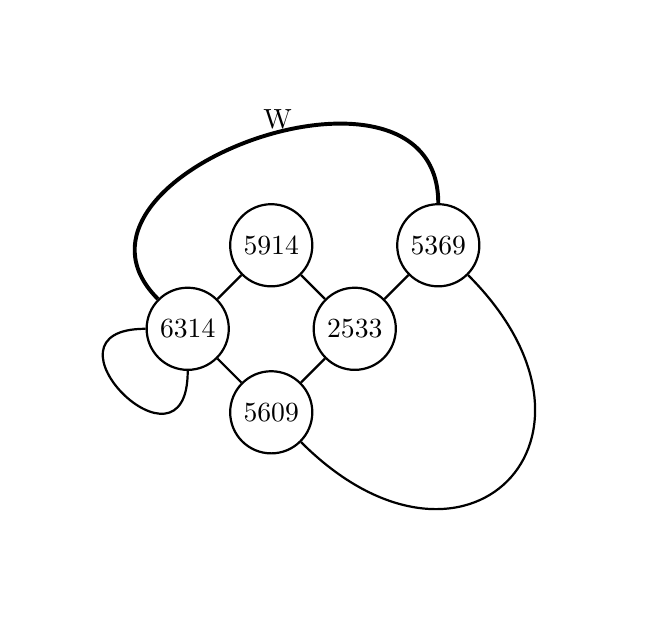
\begin{tikzpicture}[node distance={15mm}, thick, main/.style = {draw, circle}] 
\node[main] (1) {$6314$}; 
\node[main] (2) [above right of=1] {$5914$}; 
\node[main] (3) [below right of=1] {$5609$}; 
\node[main] (4) [above right of=3] {$2533$}; 
\node[main] (5) [above right of=4] {$5369$}; 

\draw(1) -- (2); 
\draw(1) -- (3); 
\draw [line width=0.05cm] (1) to [out=135,in=90,looseness=1.5] node[midway, above right] {W}  (5); 
\draw (1) to [out=180,in=270,looseness=5] (1); 
\draw (2) -- (4); 
\draw (3) -- (4); 
\draw (5) -- (4); 
\draw (5) to [out=315, in=315, looseness=2.5]  (3); 

\end{tikzpicture} 
\caption{Seismic Network (Graph representation) example: Nodes are identified as $cubeIndex$. This indexing makes it easy to acces any information about events in that respective cube from our Earthquakes Table. Also, if the network is weighted, this can be represented on the edge as $W$, where each additional link between two nodes increases this value by 1.}
\end{figure}

So now we posses the two fundamental tools used in our following analysis, the earthquakes table and the seismic network


%---------------------------------------------------------------
\section{Centrality Measures of a Network}
The fundamental measure to describe our seismic network is the connectivity distribution $P(k)$ \cite{latora}. This distribution comes naturally by realising the histogram of the nodes degree and computing the distribution. We also fit the log-log plot of this distribution and show that it is scale-free.

\begin{equation}
P(k) \sim k^{-\gamma}
\end{equation}

The connectivity computations are made for various seismic networks (Vrancea(Romania), California(USA), Italy and Japan), with different magnitude restrictions, for 2 cube sizes: $5\times5\times5$ km and $10\times10\times10$ km, with and without edge weights.

% ---------------------------- VRANCEA CONNECTIVITY ----------------------------%
\clearpage
\paragraph{Vrancea} - Connectivity
\begin{figure}[!h]
\begin{subfigure}{.99\textwidth}
  \centering
  \includegraphics[width=.85\columnwidth]{connectivityVrancea_1magnitude10}
  \caption{$1 \leq magnitude$}
  \label{fig:conVr1mag10}
\end{subfigure}%

\begin{subfigure}{.99\textwidth}
  \centering
  \includegraphics[width=.85\columnwidth]{connectivityVrancea_2magnitude10}
  \caption{$2 \leq magnitude$}
  \label{fig:conVr2mag10}
\end{subfigure}%

\begin{subfigure}{.99\textwidth}
  \centering
  \includegraphics[width=.85\columnwidth]{connectivityVrancea_2magnitude4}
  \caption{$2\leq magnitude \leq 4$}
  \label{fig:conVr2mag14}
\end{subfigure}%

\begin{subfigure}{.99\textwidth}
  \centering
  \includegraphics[width=.85\columnwidth]{connectivityVrancea_3magnitude7}
  \caption{$3 \leq magnitude \leq 7$}
  \label{fig:conVr3mag7}
\end{subfigure}%

\caption{Connectivity distribution $P(k)$ for Vrancea in log-log and linear interpolation of the results, for a number of magnitude ranges. For each range, two granularization sizes of the seismic areas have been chosen: on the left $5 \times 5 \times5 $ km cubes and on the right $10 \times 10 \times 10$ km cubes. The exponent of the fit, $\gamma$ ranges from $\sim 1.08$ to $1.756$.}
\label{fig:connectivityVr}
\end{figure}

\clearpage
\paragraph{Vrancea} - Connectivity Weighted
\begin{figure}[!h]
\begin{subfigure}{.99\textwidth}
  \centering
  \includegraphics[width=.85\columnwidth]{connectivityVranceaWeighted_1magnitude10}
  \caption{$1 \leq magnitude$}
  \label{fig:conWeiVr1mag10}
\end{subfigure}%

\begin{subfigure}{.99\textwidth}
  \centering
  \includegraphics[width=.85\columnwidth]{connectivityVranceaWeighted_2magnitude10}
  \caption{$2 \leq magnitude$}
  \label{fig:conWeiVr2mag10}
\end{subfigure}%

\begin{subfigure}{.99\textwidth}
  \centering
  \includegraphics[width=.85\columnwidth]{connectivityVranceaWeighted_2magnitude4}
  \caption{$2\leq magnitude \leq 4$}
  \label{fig:conWeiVr2mag4}
\end{subfigure}%

\begin{subfigure}{.99\textwidth}
  \centering
  \includegraphics[width=.85\columnwidth]{connectivityVranceaWeighted_3magnitude7}
  \caption{$3 \leq magnitude \leq 7$}
  \label{fig:conWeiVr3mag7}
\end{subfigure}%

\caption{Weighted connectivity distribution $P(k)$ for Vrancea in log-log and linear interpolation of the results, for a number of magnitude ranges. For each range, two granularization sizes of the seismic areas have been chosen: on the left $5 \times 5 \times5 $ km cubes and on the right $10 \times 10 \times 10$ km cubes. The exponent of the fit, $\gamma$ ranges from $\sim 1.95$ to $3.26$.}
\label{fig:connectivityVrWeighted}
\end{figure}


% ---------------------------- California CONNECTIVITY ----------------------------%
\clearpage
\paragraph{California} - Connectivity
\begin{figure}[!h]
\begin{subfigure}{.99\textwidth}
  \centering
  \includegraphics[width=.85\columnwidth]{connectivityCalifornia_1magnitude10}
  \caption{$1 \leq magnitude$}
  \label{fig:conCa1mag10}
\end{subfigure}%

\begin{subfigure}{.99\textwidth}
  \centering
  \includegraphics[width=.85\columnwidth]{connectivityCalifornia_2magnitude10}
  \caption{$2\leq magnitude$}
  \label{fig:conCa2mag10}
\end{subfigure}%

\begin{subfigure}{.99\textwidth}
  \centering
  \includegraphics[width=.85\columnwidth]{connectivityCalifornia_1magnitude3}
  \caption{$1 \leq magnitude \leq 3$}
  \label{fig:conCa1mag3}
\end{subfigure}%

\begin{subfigure}{.99\textwidth}
  \centering
  \includegraphics[width=.85\columnwidth]{connectivityCalifornia_2magnitude4}
  \caption{$2 \leq magnitude \leq 4$}
  \label{fig:conCa2mag4}
\end{subfigure}%

\caption{Connectivity distribution $P(k)$ for California in log-log and linear interpolation of the results, for a number of magnitude ranges. For each range, two granularization sizes of the seismic areas have been chosen: on the left $5 \times 5 \times5 $ km cubes and on the right $10 \times 10 \times 10$ km cubes. The exponent of the fit, $\gamma$ ranges from $\sim 1.45$ to $2.16$.}
\label{fig:connectivityCa}
\end{figure}

\clearpage
\paragraph{California} - Connectivity Weighted
\begin{figure}[!h]
\begin{subfigure}{.99\textwidth}
  \centering
  \includegraphics[width=.85\columnwidth]{connectivityCaliforniaWeighted_1magnitude10}
  \caption{$1 \leq magnitude$}
  \label{fig:conWeiCa1mag10}
\end{subfigure}%

\begin{subfigure}{.99\textwidth}
  \centering
  \includegraphics[width=.85\columnwidth]{connectivityCaliforniaWeighted_2magnitude10}
  \caption{$2\leq magnitude$}
  \label{fig:conWeiCa2mag10}
\end{subfigure}%

\begin{subfigure}{.99\textwidth}
  \centering
  \includegraphics[width=.85\columnwidth]{connectivityCaliforniaWeighted_1magnitude3}
  \caption{$1 \leq magnitude \leq 3$}
  \label{fig:conWeiCa1mag3}
\end{subfigure}%

\begin{subfigure}{.99\textwidth}
  \centering
  \includegraphics[width=.85\columnwidth]{connectivityCaliforniaWeighted_2magnitude4}
  \caption{$2 \leq magnitude \leq 4$}
  \label{fig:conWeiCa2mag4}
\end{subfigure}%


\caption{Weighted connectivity distribution $P(k)$ for California in log-log and linear interpolation of the results, for a number of magnitude ranges. For each range, two granularization sizes of the seismic areas have been chosen: on the left $5 \times 5 \times5 $ km cubes and on the right $10 \times 10 \times 10$ km cubes. The exponent of the fit, $\gamma$ ranges from $\sim 2.06$ to $2.71$.}
\label{fig:connectivityCaWeighted}
\end{figure}


% ---------------------------- Italy CONNECTIVITY ----------------------------%
\clearpage
\paragraph{Italy} - Connectivity
\begin{figure}[!h]
\begin{subfigure}{.99\textwidth}
  \centering
  \includegraphics[width=.85\columnwidth]{connectivityItaly_1magnitude10}
  \caption{$1 \leq magnitude$}
  \label{fig:conIt1mag10}
\end{subfigure}%

\begin{subfigure}{.99\textwidth}
  \centering
  \includegraphics[width=.85\columnwidth]{connectivityItaly_2magnitude10}
  \caption{$2\leq magnitude$}
  \label{fig:conIt2mag10}
\end{subfigure}%

\begin{subfigure}{.99\textwidth}
  \centering
  \includegraphics[width=.85\columnwidth]{connectivityItaly_1magnitude3}
  \caption{$1 \leq magnitude \leq 3$}
  \label{fig:conIt1mag3}
\end{subfigure}%

\begin{subfigure}{.99\textwidth}
  \centering
  \includegraphics[width=.85\columnwidth]{connectivityItaly_2magnitude4}
  \caption{$2 \leq magnitude \leq 4$}
  \label{fig:conIt2mag4}
\end{subfigure}%

\caption{Connectivity distribution $P(k)$ for Italy in log-log and linear interpolation of the results, for a number of magnitude ranges. For each range, two granularization sizes of the seismic areas have been chosen: on the left $5 \times 5 \times5 $ km cubes and on the right $10 \times 10 \times 10$ km cubes. The exponent of the fit, $\gamma$ ranges from $\sim 1.44$ to $2.3$.}
\label{fig:connectivityIt}
\end{figure}

\clearpage
\paragraph{Italy} - Connectivity Weighted
\begin{figure}[!h]
\begin{subfigure}{.99\textwidth}
  \centering
  \includegraphics[width=.85\columnwidth]{connectivityItalyWeighted_1magnitude10}
  \caption{$1 \leq magnitude$}
  \label{fig:conWeiIt1mag10}
\end{subfigure}%

\begin{subfigure}{.99\textwidth}
  \centering
  \includegraphics[width=.85\columnwidth]{connectivityItalyWeighted_2magnitude10}
  \caption{$1 \leq magnitude$}
  \label{fig:conWeiIt2mag10}
\end{subfigure}%

\begin{subfigure}{.99\textwidth}
  \centering
  \includegraphics[width=.85\columnwidth]{connectivityItalyWeighted_1magnitude3}
  \caption{$1 \leq magnitude \leq 3$}
  \label{fig:conWeiIt1mag3}
\end{subfigure}%

\begin{subfigure}{.99\textwidth}
  \centering
  \includegraphics[width=.85\columnwidth]{connectivityItalyWeighted_2magnitude4}
  \caption{$2 \leq magnitude \leq 4$}
  \label{fig:conWeiIt2mag4}
\end{subfigure}%

\caption{Weighted connectivity distribution $P(k)$ for Italy in log-log and linear interpolation of the results, for a number of magnitude ranges. For each range, two granularization sizes of the seismic areas have been chosen: on the left $5 \times 5 \times5 $ km cubes and on the right $10 \times 10 \times 10$ km cubes. The exponent of the fit, $\gamma$ ranges from $\sim 2.8$ to $3.72$.}
\label{fig:connectivityItWeighted}
\end{figure}


% ---------------------------- Japan CONNECTIVITY ----------------------------%
\clearpage
\paragraph{Japan} - Connectivity
\begin{figure}[!h]
\begin{subfigure}{.99\textwidth}
  \centering
  \includegraphics[width=.85\columnwidth]{connectivityJapan_1magnitude10}
  \caption{$1 \leq magnitude$}
  \label{fig:conJa1mag10}
\end{subfigure}%

\begin{subfigure}{.99\textwidth}
  \centering
  \includegraphics[width=.85\columnwidth]{connectivityJapan_2magnitude10}
  \caption{$2\leq magnitude$}
  \label{fig:conJa2mag10}
\end{subfigure}%

\begin{subfigure}{.99\textwidth}
  \centering
  \includegraphics[width=.85\columnwidth]{connectivityJapan_1magnitude3}
  \caption{$1 \leq magnitude \leq 3$}
  \label{fig:conJa1mag3}
\end{subfigure}%

\begin{subfigure}{.99\textwidth}
  \centering
  \includegraphics[width=.85\columnwidth]{connectivityJapan_2magnitude4}
  \caption{$2 \leq magnitude \leq 4$}
  \label{fig:conJa2mag4}
\end{subfigure}%

\caption{Connectivity distribution $P(k)$ for Japan in log-log and linear interpolation of the results, for a number of magnitude ranges. For each range, two granularization sizes of the seismic areas have been chosen: on the left $5 \times 5 \times5 $ km cubes and on the right $10 \times 10 \times 10$ km cubes. The exponent of the fit, $\gamma$ ranges from $\sim 1.87$ to $2.5$.}
\label{fig:connectivityJa}
\end{figure}

\clearpage
\paragraph{Japan} - Connectivity Weighted
\begin{figure}[!h]
\begin{subfigure}{.99\textwidth}
  \centering
  \includegraphics[width=.85\columnwidth]{connectivityJapanWeighted_1magnitude10}
  \caption{$1 \leq magnitude$}
  \label{fig:conWeiJa1mag10}
\end{subfigure}%

\begin{subfigure}{.99\textwidth}
  \centering
  \includegraphics[width=.85\columnwidth]{connectivityJapanWeighted_2magnitude10}
  \caption{$2\leq magnitude$}
  \label{fig:conWeiJa2mag10}
\end{subfigure}%

\begin{subfigure}{.99\textwidth}
  \centering
  \includegraphics[width=.85\columnwidth]{connectivityJapanWeighted_1magnitude3}
  \caption{$1\leq magnitude \leq 3$}
  \label{fig:conWeiJa1mag3}
\end{subfigure}%

\begin{subfigure}{.99\textwidth}
  \centering
  \includegraphics[width=.85\columnwidth]{connectivityJapanWeighted_2magnitude4}
  \caption{$2 \leq magnitude \leq 4$}
  \label{fig:conWeiJa2mag4}
\end{subfigure}%

\caption{Weighted connectivity distribution $P(k)$ for Japan in log-log and linear interpolation of the results, for a number of magnitude ranges. For each range, two granularization sizes of the seismic areas have been chosen: on the left $5 \times 5 \times5 $ km cubes and on the right $10 \times 10 \times 10$ km cubes. The exponent of the fit, $\gamma$ ranges from $\sim 2.45$ to $3.17$.}
\label{fig:connectivityItWeighted}
\end{figure}


\clearpage
%---------------------------------------------------------------
\section{Network Cycles and Motifs}
In this section the general approach to define and detect the building blocks of a network is being described \cite{latora}.\par 
In social and biological networks it has been noticed that triangles are highly recurrent, so work has been done in identifying where and why these kind of patterns appear. They are generally called {\it cycles} of different lengths $C_l$ and other subgraphs known as {\it motifs} $F_{n,l}$, which represent cycles that occur in {\it real networks} more frequently than in their corresponding random counterparts.


%----------%--------------%---------------------------------
\subsection{Motifs}
Network motifs are sub-graphs that repeat themselves in a specific network or even among various networks. Each of these sub-graphs, defined by a particular pattern of interactions between vertices, may reflect a framework in which particular functions are achieved efficiently. They have gathered much attention as a useful concept to uncover structural and functional design principles of complex networks. In bioinformatics, network motifs have been applied to various applications including prediction of protein interactions, identifying breast cancer related genes, and detection of essential proteins. Although network motifs may provide a deep insight into the network's functional abilities, their detection is computationally challenging.\par 

Given an undirected graph $G=(\mathcal{N},\mathcal{L})$ and any possible small connected graph $F_{n,l}$ with $n$ nodes and $l$ links, we wish to find out if $F$ is a significant subgraph of $G$. This is done by comparing the number of subgraphs of $G$ isomorphic to $F$ with the number of subraphs of a randomised network $G'=(\mathcal{N},\mathcal{L})$ isomorphic to $F$.\\
The simplest approach to quantify the relevance of $F_{n,l}$ as a subgraph of $G$ is based on the evaluation of the {\it Z-score}, defined as follows:
\begin{equation}
Z_F = \frac{n_f - \bar{n}^{rand}_F}{\sigma_{n_F}^{rand}}
\end{equation}
where $n_F$ is the number of times the subgraph $F_{n,l}$ appears in $G$ and $\bar{n}^{rand}_F$ and $\sigma_{n_F}^{rand}$ are the mean and the standard deviation, respectively, of the number of occurences in an ensemble of graphs obtained by randomising $G$.\par 
The absolute value of $Z_F$ indicates the distance between observed number of occurences and expected number of occurences in a corresponding ensemble of randomized networks with $N$ and $K$ equal to those of our network $G$, in units of standard deviations. We are interested in values of $Z_F$ larger than 2, meaning that the number of occurences is two standard deviations larger than $\bar{n}^{rand}_F$, which is a good indicator that the observed number of occurences are due to fluctuations only in $2.14\%$. Even better, when $Z_F=3$, the percentage drops to $0.13\%$, so a very good indication that $F_{n,l}$ is a network motif.


%----------%--------------%---------------------------------
\subsection{Motifs detection using NemoSuite}
NemoSuite \cite{nemosuite} (Network Motif Analysis in a Suite) is a web program developed and hosted online by researchers at University of Washington Bothell CSSE to detect and analyze network motifs. A network motif is a frequent and unique subgraph pattern in an input network, and it is determined by P-value beings smaller than 0.05 or Z-score being larger than 2.\par 

Network motif detection methods can be categorized into {\it network-centric} and {\it motif-centric} methods:
\begin{itemize}
	\item {\bf Nemo}: {\it Network-centric} approach searches all possible non-isomorphic subgraph patterns with a size (typically 3 to 8) and determines a pattern as a motif if the frequency of it is relatively high compared in a corresponding random graph. The network-centric motif detection program improves an ESU (Enumerate SUbgraphs) algorithm introduced by Sebastian Wernicke \cite{ESUmotifs} and has more functionality and output formats (NemoCount, NemoProfile, and NemoCollect). We are interested in these for the instance collection capability.
	
	\item {\bf NemoMapPy}: {\it Motif-centric} approach determines whether the given subgraph pattern is network motif by providing its frequency in an input network. Motif-centric method can determine large size of network motifs (typically larger than 8) by focusing on searching the given pattern. The program implements the NemoMap \cite{nemomap} algorithm developed by the same group and ported to python, which is based on Grochow and Kellis algorithm \cite{GK} and MODA program \cite{MODA}.
\end{itemize}


After creating the seismic network as described in \ref{subsection:seismicNetwork}, for different magnitude restrictions, we used the NemoSuite web application to identify and collect the 3 and 4 nodes motifs (triangles and tetrahedrons) in the network.\par
 Having the motif nodes, our goal is to plot the distribution of the surfaces (for the 3 nodes motifs) and volumes (for the 4 nodes motifs) weighted by the mean and total energy released by the earthquakes in the cubes that form each motif.

\clearpage
%----------%--------------%---------------------------------
\subsection{Triangle Surfaces}
For the 3 nodes motifs, calculations proceeds as follows:
\begin{itemize}

	\item Firstly we need to calculate the mean energy in each motif. The NemoSuite application \cite{nemosuite} extracts the node names of each motif from our network and using the "earthquakes list" attribute of each node we can identify every earthquake in each motif. Using the earthquakes table we can compute the {\it total energy} release of the earthquakes in each triangle, and by dividing by the total number of earthquakes in the motif we obtain the {\it mean energy} released.
	
	\item Then we use the motif nodes to calculate the surface of each motif. By having the geographical coordinates of each node, we use python's geopy library to calculate the exact "flat" distance along geodesic between two points using latitude and longitude in kilometers, and then we use pythagorean theorem to calculate the distance between the points, including the depth. Example for two points $X(lat,long,depth)$ and $Y(lat2,long2,depth2)$, $XY$ being the side of the respectie triangle:
	\begin{equation}
	\begin{split}
	&flatDistance = distance(X(lat,long),Y(lat2,long2)).km,\\
	&distance().km = \text{geopy distance function in km},\\
	&XY = \sqrt{flatDistance^2 +(X(depth)-Y(depth2))^2.}
	\end{split}
	\end{equation}
	
	\item After calculating all 3 sides of the triangle, we use Heron's formula for triangle surface:
	\begin{equation}
	\begin{split}
	&S = \sqrt{sp*(sp-a)*(sp-b)*(sp-c)},  \\
	&sp = \frac{a+b+c}{2}, \\
	&a,b,c = \text{the sides of the triangle}.
	\end{split}
	\end{equation}	
	
	\item We use the mean and total energy release per motif and the motif's surface to calculate the distribution of motifs surfaces weighted by mean or total energy.
	
	\item Compute the regression of the distribution in log-log space.
\end{itemize}

The computations are made for various seismic networks (Vrancea(Romania), California(USA) and Italy), with different magnitude restrictions, for 2 cube sizes: $5\times5\times5$ km and $10\times10\times10$ km.

% ---------------------- VRANCEA TRIANGLES -------------------

\clearpage
\paragraph{Vrancea} Mean Energy Weighted Surfaces
\begin{figure}[h!]
\begin{subfigure}{.99\textwidth}
  \centering
  \includegraphics[width=.85\columnwidth]{quakesVrancea_meanEnergy_1mag_trianglesAreas}
  \caption{$1 \leq magnitude$}
  \label{fig:trianglesVrME1}
\end{subfigure}%

\begin{subfigure}{.99\textwidth}
  \centering
  \includegraphics[width=.85\columnwidth]{quakesVrancea_meanEnergy_2mag_trianglesAreas}
  \caption{$2 \leq magnitude$}
  \label{fig:trianglesVrME2}
\end{subfigure}%

\begin{subfigure}{.99\textwidth}
  \centering
  \includegraphics[width=.85\columnwidth]{quakesVrancea_meanEnergy_3mag_trianglesAreas}
  \caption{$3 \leq magnitude$}
  \label{fig:trianglesVrME3}
\end{subfigure}%

\caption{$S_{ME} = Surface/Mean$ $Energy$ distribution in log-log plots for triangle motifs in Vrancea for 3 magnitude restrictions. The resulting interpolation shows that the distribution appears scale-free with $\gamma$ ranging from $\sim 1.14$ to $2.1$ }
\label{fig:trianglesSurfacesVrME}
\end{figure}


\clearpage
\paragraph{Vrancea} - Total Energy Weighted Surfaces
\begin{figure}[h!]

\begin{subfigure}{.99\textwidth}
  \centering
  \includegraphics[width=.85\columnwidth]{quakesVrancea_totalEnergy_1mag_trianglesAreas}
  \caption{$1 \leq magnitude$}
  \label{fig:trianglesVrTE1}
\end{subfigure}%

\begin{subfigure}{.99\textwidth}
  \centering
  \includegraphics[width=.85\columnwidth]{quakesVrancea_totalEnergy_2mag_trianglesAreas}
  \caption{$2 \leq magnitude$}
  \label{fig:trianglesVrTE2}
\end{subfigure}%

\begin{subfigure}{.99\textwidth}
  \centering
  \includegraphics[width=.85\columnwidth]{quakesVrancea_totalEnergy_3mag_trianglesAreas}
  \caption{$3 \leq magnitude$}
  \label{fig:trianglesVrTe3}
\end{subfigure}%

\caption{$S_{TE} = Surface/Total$ $Energy$ distribution in log-log plots for triangle motifs in Vrancea for 3 magnitude restrictions. The resulting interpolation shows that the distribution appears scale-free with $\gamma$ ranging from $\sim 2.79$ to $3.67$ }
\label{fig:trianglesSurfacesVrTE}
\end{figure}


\clearpage
% ---------------------- CALIFORNIA TRIANGLES -------------------____%
\paragraph{California} - Mean Energy Weighted Surfaces
\begin{figure}[h!]

\begin{subfigure}{.99\textwidth}
  \centering
  \includegraphics[width=.85\columnwidth]{quakesCalifornia_meanEnergy_2mag_trianglesAreas}
  \caption{$2 \leq magnitude$}
  \label{fig:trianglesCaME2}
\end{subfigure}%

\begin{subfigure}{.99\textwidth}
  \centering
  \includegraphics[width=.85\columnwidth]{quakesCalifornia_meanEnergy_3mag_trianglesAreas}
  \caption{$3 \leq magnitude$}
  \label{fig:trianglesCaME3}
\end{subfigure}%

\caption{$S_{ME} = Surface/Mean$ $Energy$ distribution in log-log plots for triangle motifs in California for 2 magnitude restrictions. The resulting interpolation shows that the distribution appears scale-free with $\gamma$ ranging from $\sim 1.42$ to $4.46$}
\label{fig:trianglesSurfacesCaME}
\end{figure}


\clearpage
\paragraph{California} - Total Energy Weighted Surfaces
\begin{figure}[h!]

\begin{subfigure}{.99\textwidth}
  \centering
  \includegraphics[width=.85\columnwidth]{quakesCalifornia_totalEnergy_2mag_trianglesAreas}
  \caption{$2 \leq magnitude$}
  \label{fig:trianglesCaTE2}
\end{subfigure}%

\begin{subfigure}{.99\textwidth}
  \centering
  \includegraphics[width=.85\columnwidth]{quakesCalifornia_totalEnergy_3mag_trianglesAreas}
  \caption{$3 \leq magnitude$}
  \label{fig:trianglesCaTe3}
\end{subfigure}%

\caption{$S_{TE} = Surface/Total$ $Energy$ distribution in log-log plots for triangle motifs in California for 2 magnitude restrictions. The resulting interpolation shows that the distribution appears scale-free with $\gamma$ ranging from $\sim 2.56$ to $5.01$ }
\label{fig:trianglesSurfacesCaTE}
\end{figure}


\clearpage
% ---------------------- Italy TRIANGLES -------------------____%
\paragraph{Italy} - Mean Energy Weighted Surfaces
\begin{figure}[h!]

%\begin{subfigure}{.99\textwidth}
  \centering
  \includegraphics[width=.85\columnwidth]{quakesItaly_meanEnergy_2mag_trianglesAreas}
  \caption{$2 \leq magnitude$}
  \label{fig:trianglesItME2}
%\end{subfigure}%

%\begin{subfigure}{.99\textwidth}
%  \centering
%  \includegraphics[width=.85\columnwidth]{quakesItaly_meanEnergy_3mag_trianglesAreas}
%  \caption{$3 \leq magnitude$}
%  \label{fig:trianglesItME3}
%\end{subfigure}%

\caption{$S_{ME} = Surface/Mean$ $Energy$ distribution in log-log plots for triangle motifs in Italy for $2 \leq magnitude$. The resulting interpolation shows that the distribution appears scale-free better at 10 km cube side granularization, with $\gamma = 1.503$ }
\label{fig:trianglesSurfacesItME}
\end{figure}


\paragraph{Italy} - Total Energy Weighted Surfaces
\begin{figure}[h!]

%\begin{subfigure}{.99\textwidth}
  \centering
  \includegraphics[width=.85\columnwidth]{quakesItaly_totalEnergy_2mag_trianglesAreas}
%  \caption{$2 \leq magnitude$}
  \label{fig:trianglesItTE2}
%\end{subfigure}%

%\begin{subfigure}{.99\textwidth}
%  \centering
%  \includegraphics[width=.85\columnwidth]{quakesItaly_totalEnergy_3mag_trianglesAreas}
%  \caption{$3 \leq magnitude$}
%  \label{fig:trianglesItTe3}
%\end{subfigure}%

\caption{$S_{TE} = Surface/Total$ $Energy$ distribution in log-log plots for triangle motifs in Italy for $2 \leq magnitude$. The resulting interpolation shows that the distribution appears scale-free better at 10 km cube side granularization, with $\gamma = 3.44$}
\label{fig:trianglesSurfacesItTE}
\end{figure}

\clearpage
%----------%--------------%---------------------------------
\subsection{Tetrahedrons Volumes}
For the 4 nodes motifs, calculations proceeds as follows:
\begin{itemize}

	\item The first two steps, calculation of mean energy per motif and all the sides of the tetrahedron are similar with the triangles
	
	\item For the volume, we use the Heron-like formula \cite{tetrahedron} for tetrahedrons:
	\begin{equation}
	\begin{split}
	&A = (w-U+v)*(U+v+w),a = (U-v+w)*(v-w+U)\\
    &B = (u-V+w)*(V+w+u),b = (V-w+u)*(w-u+V)\\
    &C = (v-W+u)*(W+u+v),c = (W-u+v)*(u-v+W)\\
    &W,V,U,u,v,w = \text{the sides of the tetrahedron}\\
    &p=\sqrt{a*B*C},q=\sqrt{b*C*A},r=\sqrt{c*A*B},s=\sqrt{a*b*c}\\
    &V=\frac{\sqrt{(-p+q+r+s)*(p-q+r+s)*(p+q-r+s)*(p+q+r-s)}}{192*u*v*w}
	\end{split}
	\end{equation}
	
	\item We use the mean and total energy release per motif and the motif's volume to calculate the distribution of motifs volumes weighted by mean or total energy.
	
	\item Compute the regression of the distribution in log-log space.
\end{itemize}

The computations are made for various seismic networks (Vrancea(Romania), California(USA) and Italy), with different magnitude restrictions, for 2 cube sizes: $5\times5\times5$ km and $10\times10\times10$ km.

\clearpage
%------------%----------_ VRANCEA SQUARES ---------------%
\paragraph{Vrancea} Mean Energy Weighted Volumes
\begin{figure}[!h]
\begin{subfigure}{.99\textwidth}
  \centering
  \includegraphics[width=.85\columnwidth]{quakesVrancea_meanEnergy_1mag_squaresVolumes}
  \caption{$1 \leq magnitude$}
  \label{fig:volumesVrME1}
\end{subfigure}%

\begin{subfigure}{.99\textwidth}
  \centering
  \includegraphics[width=.85\columnwidth]{quakesVrancea_meanEnergy_2mag_squaresVolumes}
  \caption{$2 \leq magnitude$}
  \label{fig:volumesVrME2}
\end{subfigure}%

\begin{subfigure}{.99\textwidth}
  \centering
  \includegraphics[width=.85\columnwidth]{quakesVrancea_meanEnergy_3mag_squaresVolumes}
  \caption{$3 \leq magnitude$}
  \label{fig:volumesVrME3}
\end{subfigure}%

\caption{$V_{ME} = Volume/Mean$ $Energy$ distribution in log-log plots for tetrahedron motifs in Vrancea for 3 magnitude restrictions. The resulting interpolation shows that the distribution appears scale-free with $\gamma$ ranging from $\sim 1.44$ to $2.8$}
\label{fig:tetrahedronsVolumesVrME}
\end{figure}

\clearpage
\paragraph{Vrancea} Total Energy Weighted Volumes
\begin{figure}[!h]
\begin{subfigure}{.99\textwidth}
  \centering
  \includegraphics[width=.85\columnwidth]{quakesVrancea_totalEnergy_1mag_squaresVolumes}
  \caption{$1 \leq magnitude$}
  \label{fig:volumesVrTE1}
\end{subfigure}%

\begin{subfigure}{.99\textwidth}
  \centering
  \includegraphics[width=.85\columnwidth]{quakesVrancea_totalEnergy_2mag_squaresVolumes}
  \caption{$2 \leq magnitude$}
  \label{fig:volumesVrTE2}
\end{subfigure}%

\begin{subfigure}{.99\textwidth}
  \centering
  \includegraphics[width=.85\columnwidth]{quakesVrancea_totalEnergy_3mag_squaresVolumes}
  \caption{$3 \leq magnitude$}
  \label{fig:volumesVrTE3}
\end{subfigure}%

\caption{$V_{TE} = Volume/Total$ $Energy$ distribution in log-log plots for tetrahedron motifs in Vrancea for 3 magnitude restrictions. The resulting interpolation shows that the distribution appears scale-free with $\gamma$ ranging from $\sim 2.94$ to $4.77$}
\label{fig:tetrahedronsVolumesVrTE}
\end{figure}

\clearpage

%------------%----------_ CALIFORNIA SQUARES ---------------%
\paragraph{California} Mean Energy Weighted Volumes
\begin{figure}[!h]

%\begin{subfigure}{.99\textwidth}
  \centering
  \includegraphics[width=.85\columnwidth]{quakesCalifornia_meanEnergy_3mag_squaresVolumes}
%  \caption{$3 \leq magnitude$}
%  \label{fig:volumesCaME3}
%\end{subfigure}%

\caption{$V_{ME} = Volume/Mean$ $Energy$ distribution in log-log plots for tetrahedron motifs in California for $3 \leq magnitude$. The resulting interpolation shows that the distribution appears scale-free better at 10 km cube side granularization, with $\gamma = 1.835$}
\label{fig:tetrahedronsVolumesCaME}
\end{figure}


\paragraph{California} Total Energy Weighted Volumes
\begin{figure}[!h]

%\begin{subfigure}{.99\textwidth}
  \centering
  \includegraphics[width=.85\columnwidth]{quakesCalifornia_totalEnergy_3mag_squaresVolumes}
%  \caption{$3 \leq magnitude$}
%  \label{fig:volumesCaTE3}
%\end{subfigure}%

\caption{$V_{TE} = Volume/Total$ $Energy$ distribution in log-log plots for tetrahedron motifs in California for $3 \leq magnitude$. The resulting interpolation shows that the distribution appears scale-free better at 10 km cube side granularization, with $\gamma = 3.156$}
\label{fig:tetrahedronsVolumesCaTE}
\end{figure}


%------------%----------_ Italy SQUARES ---------------%
\paragraph{Italy} Mean Energy Weighted Volumes
\begin{figure}[!h]

%\begin{subfigure}{.99\textwidth}
  \centering
  \includegraphics[width=.85\columnwidth]{quakesItaly_meanEnergy_3mag_squaresVolumes}
%  \caption{$3 \leq magnitude$}
%  \label{fig:volumesItE3}
%\end{subfigure}%

\caption{$V_{ME} = Volume/Mean$ $Energy$ distribution in log-log plots for tetrahedron motifs in Italy for $3 \leq magnitude$. The resulting interpolation shows that the distribution appears scale-free  better at 10 km cube side granularization, with $\gamma = 3.371$}
\label{fig:tetrahedronsVolumesItME}
\end{figure}

%\clearpage
%\paragraph{Italy} Total Energy Weighted Volumes
%\begin{figure}[!h]

%\begin{subfigure}{.99\textwidth}
%  \centering
%  \includegraphics[width=.85\columnwidth]{quakesItaly_totalEnergy_3mag_squaresVolumes}
%  \caption{$3 \leq magnitude$}
%  \label{fig:volumesItTE3}
%\end{subfigure}%

%\caption{$V_{TE} = Volume/Total$ $Energy$ distribution in log-log plots for tetrahedron motifs in Italy for $3 \leq magnitude$. The resulting interpolation shows that the distribution appears scale-free with $\gamma$ ranging from $\sim 4.76$ to $6.85$}
%\label{fig:tetrahedronsVolumesItTE}
%\end{figure}


\clearpage
%--------------------------------------------------------------------
\section{Motifs Visualization}
As a visualization tool for the earthquakes networks and their motifs we used the application ParaView, which works together with the python library "VTK".\par
The Visualization ToolKit (VTK) is an open source software system for 3D graphics, visualization and image processing. VTK supports a variety of visualization algorithms : scalar, vector, tensor, texture and volumetric methods, making it easy to translate graphs into geometric form.\par
ParaView \cite{paraview} is an open-source application designed to visualize data of varying sizes, from small to very large. Under the hood, ParaView uses VTK as the data processing and rendering engine.\par 
In python, we created our graphs using the library "networkx" for it's easy and intuitive graph creation method, and easy to access node attributes using python dictionaries. The translation from networkx to vtk is fairly straight-forward: the nodes are translated as 3D Glyphs, the edges as 3D Tubes and the motifs as 3D Surfaces, using coordinates between 0 and 1 for each dimension (latitude, longitude and depth) for the vertices:
\begin{itemize}

	\item Firstly, we properly scale the coordinates of each node to fit in the [0,1] range of dimensions (needed in Paraview). Each node is represented by a geometric "Point" in vtk and each link or motif is represented by a "Cell" delimited by the proper points.
	
	\item We are also able to add scalar attributes to these geometric elements:
	\begin{itemize}
		\item for nodes: the degree of connectivity of each node;
		\item for edges : the weight of the edge and the color "quality" of the edge (0 if it's a normal edge, 1 if it's part of a motif).
	\end{itemize}
	
	\item The size of each geometric element can be adjusted according to the scalar attributes (for example, nodes with higher degree appear larger, links with larger wight appear thicker).
	
	\item The color of each geometric element can be adjusted according to the scalar attributes (for example, a gradient is applied to nodes according to their degree).
	
	\item Also the opacity of each element can be adjusted (even logarithmically, for example lower degree nodes can be less visible than higher degree nodes).
 
\end{itemize}
For visualization purposes we have chosen a smaller size network in order to properly see the geometric elements in Paraview. So, we have restricted the magnitude scale to only the events with magnitude larger than 4 (and larger than 5 for Japan).
\newpage

\paragraph{Romania} Real Network Visualization 

\begin{figure}[!h]
  \centering
  \includegraphics[width=.85\linewidth]{motifs_romania_5km_4mag_trianglesFilled}
  \caption{Motifs in Romania Seismic Network, earthquakes with magnitude $>4$. It is obviously noticed that most of the network is concentrated in the Vrancea seismic zone.}
  \label{fig:motifRomania}
\end{figure}


We can isolate only the Vrancea seismic region because that is the main area of seismicity in Romania. The coordinate restrictions are mentioned in chapter \ref{chap:quakeDatabase}. Thus we obtain a graph with 255 nodes, 375 edges, 3 triangles and 10 tetrahedrons.
\begin{figure}[!h]
\begin{subfigure}{.5\textwidth}
  \centering
  \includegraphics[width=.85\linewidth]{motifs_vrancea_5km_4mag_trianglesFilled_map}
  \caption{Triangles in Vrancea Seismic Network}
  \label{fig:motifTriangleVrancea}
\end{subfigure}%
\begin{subfigure}{.5\textwidth}
  \centering
  \includegraphics[width=.85\linewidth]{motifs_vrancea_5km_4mag_squaresFilled_map}
  \caption{Tetrahedrons in Vrancea Seismic Network}
  \label{fig:motifTetrahedronVrancea}
\end{subfigure}
\caption{Motifs in Vrancea Seismic Network - 380 events stored in 255 nodes and connected through 375 edges. The degree of connectivity of the nodes ranges from 1 to 16. The motifs are represented as surfaces, for the triangles, or by volumes for the tetrahedrons (drawn in red)}
\label{fig:volumesVrancea}
\end{figure}


\clearpage
\paragraph{California}  Real Network Visualization 

\begin{figure}[!h]
  \centering
  \includegraphics[width=.85\linewidth]{motifs_california_5km_4mag_trianglesFilled_map}
  \caption{Motifs in California Seismic Network, earthquakes with magnitude $>4$ : 1119 events are stored in 718 nodes, which are connected by 1036 edges. The degree of connectivity of the nodes ranges from 1 to 19. With red surfaces the triangles of this zone are presented.}
  \label{fig:motifCalifornia}
\end{figure}


\paragraph{Italy} Real Network Visualization 

\begin{figure}[!h]
  \centering
  \includegraphics[width=.85\linewidth]{motifs_italy_5km_4mag_squaresFilled}
  \caption{Motifs in Italy Seismic Network, earthquakes with magnitude $>4$ : 1490 events are stored in 1325 nodes, which are connected by 1452 edges. The degree of connectivity of the nodes ranges from 1 to 16. With red surfaces the tetrahedrons of this zone are presented.}
  \label{fig:motifItaly}
\end{figure}

\clearpage
\paragraph{Japan} Real Network Visualization 

\begin{figure}[!h]
  \centering
  \includegraphics[width=.85\linewidth]{motifs_japan_5km_5mag_triangles}
  \caption{Motifs in Japan Seismic Network, earthquakes with magnitude $>5$ : 16948 events are stored in 14396 nodes, which are connected by 20332 edges. The degree of connectivity of the nodes ranges from 1 to 13. With red surfaces the triangles of this zone are presented.}
  \label{fig:motifJapan}
\end{figure}

{\pagestyle{empty}\cleardoublepage}
\chapter{Seismic Spatio-Temporal Autocorrelations}
\label{chap:quakeCorrelations}

%----------------------------------------------------
\section{Correlations and Autocorrelations}

Correlations represent a measure of how one value or system responds to another. There are many different types of correlation functions which can be used to determine the correlation of two random variables or systems. For example, time correlation functions are used in the theory of noise and stochastic processes in statistical physics and spectroscopy. \par 

In signal processing, the term cross-correlation represents a type of correlation function, which is a generalized form of regular linear correlation. It is used to compare different time series, allowing to see how two signals match and where the best matching occurs, so hidden patterns in a signal may be revealed.\par 

We introduced the term cross-correlation in order to understand autcorroleation, which is what we are interested in our work. The major difference between the two is that while cross-correlation is used when two {\bf different} sequences are correlated, autocorrelation means that the correlation occurs between two of the {\bf same} sequences, i.e. you correlate the signal with itself.


%----------------------------------------------------
\section{Spatial Autocorrelations}
{\bf “Everything is related to everything else, but near things are more related than distant things.”} - Waldo R. Tobler, the first law of geography. \par \bigskip

{\it Spatial autocorrelation} helps understand the degree to which one object is similar to other nearby objects. One of the most popular tests of spatial autocorrelation is the Moran's I test \cite{moran}. In the following we present how we applied this function and the results. The objects of our function represent the total energy released by the earthquakes in each of the cubes that we split our seismic region in. \par


After creating the earthquake network we can establish the spatial correlations between nodes. First we compute the total energy release of the earthquakes in each node. So each cube now has the total energy $E_{ijk}$ associated with it.\par
Next we compute the mean energy in the network:
\begin{equation}
\begin{split}
&<E> = \frac{1}{N*M*L}\sum_{i=1}^{N}\sum_{j=1}^{M}\sum_{k=1}^{L} E_{ijk},\\
&N = \text{Number of cubes in the latitude dimension},\\
&M = \text{Number of cubes in the longitude dimension},\\
&L = \text{Number of cubes in the depth dimension}.
\end{split}
\end{equation}

Then we can compute the variance that represents the distance from the central value:
\begin{equation}
var(E) = \frac{1}{N*M*L}\sum_{i=1}^{N}\sum_{j=1}^{M}\sum_{k=1}^{L} (E_{ijk} -<E>)^2.
\end{equation}

The standard deviation can thus be defined as:
\begin{equation}
\sigma_E = \sqrt{var(E)}.
\end{equation}

Then we can introduce the covariance:
\begin{equation}
cov(E,r) = \frac{1}{N*M*L}\sum_{i=1}^{N}\sum_{j=1}^{M}\sum_{k=1}^{L} \sum_{l=1}^{N}\sum_{m=1}^{M}\sum_{n=1}^{L} (E_{ijk} -<E>)(E_{lmn} -<E>).
\end{equation}
where the cube with total energy $E_{lmn}$ is situated at distance $r$ from the cube with total energy $E_{ijk}$.

Lastly, the spatial correlation index, $M2$ is defined as the ratio of the covariance to the standard deviation squared $\sigma_{E}^2$:
\begin{equation}
M2(E,r) = \frac{cov(E,r)}{\sigma^2_E}.
\end{equation}


\paragraph{Vrancea} Spatial autocorrleation function $M2(r)$ for Vrancea networks - 3 different cube sizes $5\times5\times5$ km, $10\times10\times10$ km and $20\times20\times20$ km. Each function is presented twice: the left plot is represented with the point in $M2(0)$ and on the right, without that point in order to better see the feature of the plot.




\begin{figure}[!ht]
\begin{subfigure}{.5\textwidth}
  \centering
  \includegraphics[width=.99\linewidth]{M2_V22_Vrancea_5km_1<mag<10}
  \caption{With M2(0)}
  \label{fig:corr5km}
\end{subfigure}%
\begin{subfigure}{.5\textwidth}
  \centering
  \includegraphics[width=.99\linewidth]{M2_V22_Vrancea_5km_1<mag<10_without0}
  \caption{Without M2(0)}
  \label{fig:corr5km_noZero}
\end{subfigure}
\caption{Spatial autocorrelation function $M2(r)$ for Vrancea seismic zone split into $5\times5\times5$ km cubes. $r$ represents the distance in multiples of $5$ km. The right hand plot, without the point $M2(0)$ better displays the feature of the plot}
\label{fig:spcorrVrancea5km}
\end{figure}

\begin{figure}[!ht]
\begin{subfigure}{.5\textwidth}
  \centering
  \includegraphics[width=.99\linewidth]{M2_V22_Vrancea_10km_1<mag<10}
  \caption{With M2(0)}
  \label{fig:corr10km}
\end{subfigure}%
\begin{subfigure}{.5\textwidth}
  \centering
  \includegraphics[width=.99\linewidth]{M2_V22_Vrancea_10km_1<mag<10_without0}
  \caption{Without M2(0)}
  \label{fig:corr10km_noZero}
\end{subfigure}
\caption{Spatial autocorrelation function $M2(r)$ for Vrancea seismic zone split into $10\times10\times10$ km cubes. $r$ represents the distance in multiples of $5$ km. The right hand plot, without the point $M2(0)$ better displays the feature of the plot}
\label{fig:spcorrVrancea10km}
\end{figure}

\begin{figure}[!ht]
\begin{subfigure}{.5\textwidth}
  \centering
  \includegraphics[width=.99\linewidth]{M2_V22_Vrancea_20km_1<mag<10}
  \caption{With M2(0)}
  \label{fig:corr20km}
\end{subfigure}%
\begin{subfigure}{.5\textwidth}
  \centering
  \includegraphics[width=.99\linewidth]{M2_V22_Vrancea_20km_1<mag<10_without0}
  \caption{Without M2(0)}
  \label{fig:corr20km_noZero}
\end{subfigure}
\caption{Spatial autocorrelation function $M2(r)$ for Vrancea seismic zone split into $20\times20\times20$ km cubes. $r$ represents the distance in multiples of $5$ km. The right hand plot, without the point $M2(0)$ better displays the feature of the plot}
\label{fig:spcorrVrancea20km}
\end{figure}



\clearpage
%----------------------------------------------------
\section{Temporal Autocorrelations}
In time series analysis, autocorrelation is used to correlate observations at a time step with observations at previous time steps, called {\it lags}.\par 
In general, considering a time series $y_1,...,y_n$, it's mean is:
\begin{equation}
\bar{y}=\frac{1}{n}\sum_{i=1}^n y_i.
\end{equation}
The autocovariance function at lag $k$, for $k \geq 0$, of the time series is defined by:
\begin{equation}
s_k = \frac{1}{n}\sum_{i=1}^{n-k}(y_i - \bar{y})(y_{i+k} - \bar{y}).
\end{equation}
Finally, the autocorrelation function (ACF) at lag $k$ of the time series is:
\begin{equation}
r_k = \frac{s_k}{s_0}.
\end{equation}

For our networks, we need to establish a way of defining the lags, and the quantity that is to be autocorrelated. These calculations are made as such:

\begin{itemize}
	\item Establish the time period of the network, from the first earthquake of the database to the last. For example, as mentioned in Chapter \ref{chap:quakeDatabase} the timeframe we have for our whole network in Vrancea(Romania) is 19:03:01 August 19 1976 to 00:11:55 February 28 2021, so we would have a $timeframe$ of 16263 days and 05:08:54 hours.
	\item Next we iterate through the table and find the biggest interval $dt$ between two consecutive earthquakes. 
	\item Then, by dividing the total $timeframe$ by that interval $dt$ we create a certain amount of time windows $W$, so we have split the total timeframe in equal parts and surely each part contains at least one earthquake.
	\item Place each earthquake in it's respective time window and calculate the total energy release for each time window. Now we have $E_i$ total energies (the values of our time series $y_i$) with $i = 1,2,...W$ (the lags).
\end{itemize}
Having defined our earthquake energies time series, we can now proceed to calculate the temporal autocorrelation function by adapting the formula described earlier:\par


Firstly, compute the mean energy, by summing over all time windows $W$:
\begin{equation}
\bar{E} = \frac{1}{W}\sum_{i=1}^{W}E_i.
\end{equation}

Then you can compute the autocovariance function at lag $k$, for $k>=0$, of the time series as:
\begin{equation}
s_k = \frac{1}{W-k}\sum_{i=1}^{W-k} (E_i-\bar{E})(E_{i+k}-\bar{E}).
\end{equation}

Finally, the autocorrelation function is defined as:
\begin{equation}
C(k) = \frac{s_k}{s_0}.
\end{equation}

We realised Temporal AutoCorrelation Functions (TACFs) of the earthquake energies time series on several seismic networks, for two magnitude windows: below and above $3.5$. Below are the results, with and without the point $C(0)$ in order to better recognize the feature of the plot (the point $C(0)$ is always equal to $1$).


%------------ VRANCEA CORR -%%%%%%%%%%%%
\paragraph{Vrancea} TACF Vrancea(Romania) Seismic Network

\begin{figure}[!ht]
\begin{subfigure}{.5\textwidth}
  \centering
  \includegraphics[width=.95\linewidth]{TemporalCorrelation_Vrancea_2<mag<3.5}
  \caption{With C(0)}
  \label{fig:corrVrancea2_3.5}
\end{subfigure}%
\begin{subfigure}{.5\textwidth}
  \centering
  \includegraphics[width=.95\linewidth]{TemporalCorrelation_Vrancea_2<mag<3.5_noZero}
  \caption{Without C(0)}
  \label{fig:corrVrancea2_3.5_noZero}
\end{subfigure}
\caption{Temporal Autocorrelation Function for Vrancea(Romania) for magnitude restrictions: $2<mag<3.5$. A $timeframe$ of $16263$ days $05:08:54$ hours, containing a total of $6593$ number of events, is split into $W=83$ equal windows of $dt=198$ days $05:33:45$ hours.}
\label{fig:corrVrancea2_3.5!}
\end{figure}

\begin{figure}[!ht]
\begin{subfigure}{.5\textwidth}
  \centering
  \includegraphics[width=.95\linewidth]{TemporalCorrelation_Vrancea_3.5<mag<7}
  \caption{With C(0)}
  \label{fig:corrVrancea3.5_7}
\end{subfigure}%
\begin{subfigure}{.5\textwidth}
  \centering
  \includegraphics[width=.95\linewidth]{TemporalCorrelation_Vrancea_3.5<mag<7_noZero}
  \caption{Without C(0)}
  \label{fig:corrVrancea3.5_7_noZero}
\end{subfigure}
\caption{Temporal Autocorrelation Function for Vrancea(Romania) for magnitude restrictions: $3.5<mag<7$. A $timeframe$ of $16263$ days $05:08:54$ hours, containing a total of $1411$ number of events, is split into $W=105$ equal windows of $dt=154$ days $06:10:03$ hours.}
\label{fig:corrVrancea3.5_7!}
\end{figure}


\clearpage
%------------ California CORR -%%%%%%%%%%%%
\paragraph{California} TACF California(USA) Seismic Network

\begin{figure}[!ht]
\begin{subfigure}{.5\textwidth}
  \centering
  \includegraphics[width=.95\linewidth]{TemporalCorrelation_California_2<mag<3.5}
  \caption{With C(0)}
  \label{fig:corrCalifornia2_3.5}
\end{subfigure}%
\begin{subfigure}{.5\textwidth}
  \centering
  \includegraphics[width=.95\linewidth]{TemporalCorrelation_California_2<mag<3.5_noZero}
  \caption{Without C(0)}
  \label{fig:corrCalifornia2_3.5_noZero}
\end{subfigure}
\caption{Temporal Autocorrelation Function for California(USA) for magnitude restrictions: $2<mag<3.5$. A $timeframe$ of $13514$ days $03:53:33$ hours, containing a total of $52290$ events, is split into $W=692$ equal windows of $dt=18$ days $12:30:46$ hours.}
\label{fig:corrCalifornia2_3.5!}
\end{figure}

\begin{figure}[!ht]
\begin{subfigure}{.5\textwidth}
  \centering
  \includegraphics[width=.95\linewidth]{TemporalCorrelation_California_3.5<mag<7.2}
  \caption{With C(0)}
  \label{fig:corrCalifornia3.5_7}
\end{subfigure}%
\begin{subfigure}{.5\textwidth}
  \centering
  \includegraphics[width=.95\linewidth]{TemporalCorrelation_California_3.5<mag<7.2_noZero}
  \caption{Without C(0)}
  \label{fig:corrCalifornia3.5_7_noZero}
\end{subfigure}
\caption{Temporal Autocorrelation Function for California(USA) for magnitude restrictions: $3.5<mag<7.2$. A $timeframe$ of $13514$ days $03:53:33$ hours, containing a total of $3387$ events, is split into $W=128$ equal windows of $dt=104$ days $07:15:31$ hours.}
\label{fig:corrCalifornia3.5_7!}
\end{figure}


\clearpage
%------------ Italy CORR -%%%%%%%%%%%%
\paragraph{Italy} TACF Italy Seismic Network

\begin{figure}[!ht]
\begin{subfigure}{.5\textwidth}
  \centering
  \includegraphics[width=.95\linewidth]{TemporalCorrelation_Italy_2<mag<3.5}
  \caption{With C(0)}
  \label{fig:corrItaly2_3.5}
\end{subfigure}%
\begin{subfigure}{.5\textwidth}
  \centering
  \includegraphics[width=.95\linewidth]{TemporalCorrelation_Italy_2<mag<3.5_noZero}
  \caption{Without C(0)}
  \label{fig:corrItaly2_3.5_noZero}
\end{subfigure}
\caption{Temporal Autocorrelation Function for Italy for magnitude restrictions: $2<mag<3.5$. A $timeframe$ of $12783$ days $06:18:25$ hours, containing a total of $95004$ events, is split into $W=3040$ equal windows of $dt=3$ days $04:55:28$ hours.}
\label{fig:corrItaly2_3.5!}
\end{figure}

\begin{figure}[!ht]
\begin{subfigure}{.5\textwidth}
  \centering
  \includegraphics[width=.95\linewidth]{TemporalCorrelation_Italy_3.5<mag<7}
  \caption{With C(0)}
  \label{fig:corrItaly3.5_7}
\end{subfigure}%
\begin{subfigure}{.5\textwidth}
  \centering
  \includegraphics[width=.95\linewidth]{TemporalCorrelation_Italy_3.5<mag<7_noZero}
  \caption{Without C(0)}
  \label{fig:corrItaly3.5_7_noZero}
\end{subfigure}
\caption{Temporal Autocorrelation Function for Italy for magnitude restrictions: $3.5<mag<7$. A $timeframe$ of $12783$ days $06:18:25$ hours, containing a total of $4436$ events, is split into $W=270$ equal windows of $dt=46$ days $08:43:30$ hours.}
\label{fig:corrItaly3.5_7!}
\end{figure}



\clearpage
%------------ Japan CORR -%%%%%%%%%%%%
\paragraph{Japan} ACF Japan Seismic Network

\begin{figure}[!ht]
\begin{subfigure}{.5\textwidth}
  \centering
  \includegraphics[width=.95\linewidth]{TemporalCorrelation_Japan_2<mag<3.5}
  \caption{With C(0)}
  \label{fig:corrJapan2_3.5}
\end{subfigure}%
\begin{subfigure}{.5\textwidth}
  \centering
  \includegraphics[width=.95\linewidth]{TemporalCorrelation_Japan_2<mag<3.5_noZero}
  \caption{Without C(0)}
  \label{fig:corrJapan2_3.5_noZero}
\end{subfigure}
\caption{Temporal Autocorrelation Function for Japan for magnitude restrictions: $2<mag<3.5$. A $timeframe$ of $10104$ days $22:53:49$ hours, containing a total of $618550$ events, is split into $W=6068$ equal windows of $dt=04:55:28$ hours.}
\label{fig:corrJapan2_3.5!}
\end{figure}


\begin{figure}[!ht]
\begin{subfigure}{.5\textwidth}
  \centering
  \includegraphics[width=.95\linewidth]{TemporalCorrelation_Japan_3.5<mag<9}
  \caption{With C(0)}
  \label{fig:corrJapan3.5_9}
\end{subfigure}%
\begin{subfigure}{.5\textwidth}
  \centering
  \includegraphics[width=.95\linewidth]{TemporalCorrelation_Japan_3.5<mag<9_noZero}
  \caption{Without C(0)}
  \label{fig:corrJapan3.5_9_noZero}
\end{subfigure}
\caption{Temporal Autocorrelation Function for Italy for magnitude restrictions: $3.5<mag<9$. A $timeframe$ of $10104$ days $22:53:49$ hours, containing a total of $84324$ events, is split into $W=3213$ equal windows of $dt=2$ days $03:29:02$ hours.}
\label{fig:corrJapan3.5_9!}
\end{figure}

By analyzing the TACFs for earthquakes with $2<magnitude<3.5$, the events can be interpreted as fluctuations that exhibit a chaotic behaviour and at larger magnitudes, above $3.5$, this behaviour is lost. Here, peaks are recognized at certain lags suggesting a correlation between events at certain time intervals. This can be an indication that large events are more likely than not to be separated by these time frames. For example, in Vrancea we recognize a couple of peaks at around $30$ lags, which would translate as $\sim 12.65$ years. This means that it is possible for some large events to have a $12.65$ years span between them.\par 

{\pagestyle{empty}\cleardoublepage}

\addcontentsline{toc}{chapter}{Conclusions}
\chapter*{Conclusions}
In conclusion, we have shown how to access and extract information about earthquakes from the databases available. We presented how to construct various seismic networks for regions around the globe and by measures of connectivity and motif discovery we proved that the scale-free nature of these networks is {\bf very robust}.\par 
With the help of visualization tools such as VTK and ParaView, we have shown how these network can be graphically represented in real, geographic coordinate space, with the connectivity, edge weights and motifs pictured with the help of graphs.\par 
We also computed spatial and temporal autocorrelation functions for the regions analyzed and concluded two distinct behaviours when taking into account lower magnitude, in contrast with higher magnitude earthquakes. At lower energies, events can be viewed as some kind of chaotic fluctuations, while at higher energies, some pattern may emerge. \par 
This work sustains the popular notion that earthquakes are complex systems that show self-organization to criticality behaviour. \par 
Further study can be done in this space, with the possibility of analyzing other seismic regions by employing the same computational tools used in this report. Also, from the perspective of network theory, other centrality or community measures may give insight about clusters of earthquakes, opening the possibility of splitting a region into more relevant sections. 
{\pagestyle{empty}\cleardoublepage}

% ---------- BIBLIOGRAPHY ------------------%
\printbibliography

{\pagestyle{empty}\cleardoublepage}
% ---------- APPENDIX ------------------%
\begin{appendices}
\chapter{Collecting Databases, Energy Release and Cube Splitting}

\begin{lstlisting}[language=python, frame=single, tabsize=1]  % Start your code-block
import mysql.connector
import pandas as pd
import math

def sqlCollect(condition,side,region,withCubes=True,
		enRel=False):
	mydb = mysql.connector.connect(
	host="",
	user="",
	password="",
	database="",
	auth_plugin='mysql_native_password'
	)

	mycursor = mydb.cursor()

	# Call the database with the set conditions
	mycursor.execute(condition)

	# Append the database to the result object array
	result = mycursor.fetchall()

	# Initialize our lists    
	date= []
	lat = []
	long = []
	dep = []
	mag = []

	# Append the result of sql into our lists
	for i in range(len(result)):
		date.append(result[i][0])
		lat.append(result[i][1])
		long.append(result[i][2])
		dep.append(result[i][3])
		mag.append(result[i][4])
	  
	# Force the results into float type
	lat = [float(item) for item in lat]
	long = [float(item) for item in long]
	dep = [float(item) for item in dep]
	mag = [float(item) for item in mag]
	
	# If withCubes TRUE => collect database and 
	#create cube indexes
	if withCubes:
		# Create cubes indexes for all the dimensions
		# ------------------------------------------

		# Set min max for the dimensions
		minLat = min(lat)
		maxLat = max(lat)
		minLong = min(long)
		maxLong = max(long)
		mindep = min(dep)
		maxdep = max(dep)


		# Find the no. cubes, given the size of the cube in km 
		# Depending on region, one degree lat/long differs:

		# IN VRANCEA 1 deg Lat = 111km / 1 deg Long = 79km
		if region=='Vrancea' or region=='Romania':
			longInKm = 79
		
		# IN CALI 1 deg Lat = 111km / 1 deg Long = 94km
		if region=='California':
			longInKm = 94

		# IN ITALY 1 deg Lat = 111km / 1 deg Long = 84km
		if region=='Italy':
			longInKm = 84

		# IN JAPAN 1 deg Lat = 111km / 1 deg Long = 91km
		if region=='Japan':
			longInKm = 91

		x = round((maxLat-minLat)*111 / side)
		y = round((maxLong-minLong)*longInKm / side)
		z = round((maxdep-mindep) / side)

		# Create cubes indexes for all the dimensions 
		xlat = [math.floor((i-minLat)*x/(maxLat-minLat))+1
		 for i in lat]
		ylong = [math.floor((i-minLong)*y/(maxLong-minLong))+1
		 for i in long]
		zdep = [math.floor((i-mindep)*z/(maxdep-mindep))+1
		 for i in dep ]
		cubeIndex=[]
		# and a general cubeindex for graph formation
		for i in range(len(xlat)):
			cubeIndex.append(int(str(xlat[i])+str(ylong[i])
				+str(zdep[i])))


		# Input coordinates of every cubeIndex
		cubelat=[round(minLat + (side/111)*(i-1+1/2),4)
		 for i in xlat]
		cubelong=[round(minLong + (side/longInKm)*(i-1+1/2),4)
		 for i in ylong]
		cubedep=[round(mindep + (side)*(i-1+1/2),4)
		 for i in zdep]

		# if enRel TRUE, add a column with the energy release 
		if enRel:
			enRel=[math.pow(10, 5.24 + 1.44*i) for i in mag]

			d = {'date':date,'lat':lat,'long':long,
				'dep':dep,'mag':mag, 'enRel':enRel,'x':xlat,
				'y':ylong,'z':zdep,'cubeIndex':cubeIndex,
				'cubelat':cubelat,'cubelong':cubelong,
				'cubedep':cubedep}
			return pd.DataFrame(data=d)


		else:
			# Create DataFrame
			d = {'date':date,'lat':lat,'long':long,
				'dep':dep,'mag':mag,'x':xlat,
				'y':ylong,'z':zdep,'cubeIndex':cubeIndex,
				'cubelat':cubelat,'cubelong':cubelong,
					'cubedep':cubedep}
			return pd.DataFrame(data=d)
	
	# if withCubes==False , do not create cubes 
	else:
	
		if enRel:
			enRel=[math.pow(10, 5.24 + 1.44*i) for i in mag]

			d = {'date':date,'lat':lat,'long':long,'dep':dep,
			     'mag':mag,'enRel':enRel}
			return pd.DataFrame(data=d)
		else:
			d = {'date':date,'lat':lat,'long':long,
				'dep':dep,'mag':mag}
			return pd.DataFrame(data=d)

\end{lstlisting}


\chapter{Network Creation}

\begin{lstlisting}[language=python, frame=single, tabsize=1] 
import datetime
import pandas as pd
import networkx as nx


# Takes the qk DataFrame and returns the qk network
# in networkx graph (G) with attributes:
#(cube dimensions and index of qk with same cIdx)
def graphCreation(qk,withEdgeWeight=False):

	# Create graph -  qk ONE BY ONE
	G = nx.Graph()
	# Iterate through the earthqk checking
	# for magnitude condition
	for i in range(len(qk['cIdx'])):
		# Create a node for this earthquake
		G.add_node(qk['cIdx'][i])
		# check the following earthqk chronologically
		for j in range(i+1, len(qk['cIdx'])):
			# I want only the first occurence (break at the end)
			# create a node for the target quake index
			G.add_node(qk['cIdx'][j])
			
			# Check if you need the edge weights
			if withEdgeWeight==True:
				# WITH EDGE WEIGHT
				# check to see if there is an edge between them
				if G.has_edge(qk['cIdx'][i], qk['cIdx'][j]):
					# we added this one, increase the weight by 1
					G[qk['cIdx'][i]][qk['cIdx'][j]]['weight'] += 1
					break

				else:
					# new edge. add with weight=1
					G.add_edge(qk['cIdx'][i], qk['cIdx'][j], weight=1)
					break
			else:
				# WITHOUT EDGE WEIGHT
				G.add_edge(qk['cIdx'][i], qk['cIdx'][j])
				break

	# Setup network attributes as dictionaries
	# Only dictionaries are supported by networkx
	quake_index = {}
	quake_zDepth = {}
	quake_yLongitude = {}
	quake_xLatitude = {}

	# Turn the dataframe into a dictionary, the indexing qty
	for index, row in qk.iterrows():
		
		# Create a dictionary with cIdx :[list of quake idxs]
		# if the cube has already been indexed
		if row['cIdx'] in quake_index.keys():
			# just add that event in the dictionary
			quake_index[row['cIdx']].append(str(index))
		# if not yet indexed
		else:
			# create that dictionary entry
			quake_index[row['cIdx']]=[]
			# and add that event in the dictionary
			quake_index[row['cIdx']].append(str(index))
			
		# Create dict for each dimension (cIdx : dimension)
		quake_zDepth[row['cIdx']] = str(row['z'])
		quake_yLongitude[row['cIdx']] = str(row['y'])
		quake_xLatitude[row['cIdx']] = str(row['x'])


	nx.set_node_attributes(G, quake_zDepth, 'quake_zDep')
	nx.set_node_attributes(G, quake_yLongitude, 'quake_yLong')
	nx.set_node_attributes(G, quake_xLatitude, 'quake_xLat')
	nx.set_node_attributes(G, quake_index, 'quake_index')


	# Relabel the nodes
	nodeList=[]
	for n in G.nodes():
		nodeList.append(n)

	# Create the mapping : dict with {G node value} : 
	#new value ( from 1 to n = len of G nodes )    
	mapping = {}
	for i in range(len(nodeList)):
		# i+1 to create from 1 to n ( not from 0 ) 
		mapping[nodeList[i]] = i+1

	# Create new graph with relabeled nodes
	G = nx.relabel_nodes(G, mapping)

	return(G)

\end{lstlisting}


\chapter{Connectivity}

\begin{lstlisting}[language=python, frame=single, tabsize=1] 
from quakesNetwork_graphCreation import*
from sqlCollectDatabaseWithCubes import sqlCollect

mag=1
side=5

region = Vrancea
edgeWeight = input(' Edgeweight - True / False : ')

# VRANCEA
if region=='Vrancea':
	condition=(f"SELECT * FROM romplus WHERE 
				`dateandtime`>='1976-01-01 00:00:00'"
		   f" AND `latitude`>=45.2 AND 
		   		`latitude`<=46 AND `longitude`>=26" 
		   f" AND `longitude`<=27 AND `depth`>=50 
		   		AND `depth`<=200"
		   f" AND `magnitude`>={mag}")
		   
# Collect the database and create the graph
quakes = sqlCollect(condition,side,region)
		
# Process graph and its connectivity with edge weight
if edgeWeight=='True':
	G = graphCreation(quakes,withEdgeWeight=True)
		
	# Degree
	degree_dict = dict(G.degree(G.nodes(),weight='weight'))
	connectivity=[]
	for item in degree_dict.values():
		connectivity.append(item)
# Withoud weight
else:
	G = graphCreation(quakes)
			
	# Degree
	degree_dict = dict(G.degree(G.nodes()))
	connectivity=[]
	for item in degree_dict.values():
		connectivity.append(item)
		
# Histogram of connectivity
hist, bins = np.histogram(connectivity,
    bins=round(math.sqrt(len(connectivity))));

# Create the data k,y from the hist and bins
# k = bins centers. Create empty array of the length of hist
k = np.zeros_like(hist)
# Append to it the centers of the bins
for i in range(1,len(bins)):
	k[i-1]=((bins[i]+bins[i-1])/2)

# Check for zeros in the hist list and cut both 
#k and y where the first zero occurs
for i in range(len(hist)):
	if hist[i]==0:
		y=np.array(hist[:i])
		k=np.array(k[:i])
		break
	# If there is no zeros, make y=hist (full data )
	else:
		y=hist
		
# Renormalize the ydata to 1 => P_k
P_k = np.array([float(i)/sum(y) for i in y])
# Compute the mean degree of G : k_mean
k_mean = np.dot(k,P_k)
# Compute the remaining degree distribution q_k
q = np.array([(k[i+1]*P_k[i+1])/k_mean for
	 i in range(len(k)-1)])
# Compute the entropy
H_q = -np.dot(q,np.log(q))


# Compute the power_law fit to our data 
pars, cov = curve_fit(f=power_law,xdata=k,ydata=P_k,
	maxfev=5000)
# Compute the chi_sq  of fit = sum((obs-exp)^2/exp)
chi_squared = np.sum((P_k-power_law(k,*pars))
	**2/power_law(k,*pars))


fig, ax = plt.subplots(1,2,figsize=(15,5))

# The data, scattered
plt.scatter(k,P_k)
plt.set_xscale('log')
plt.set_yscale('log')
# The fit
plt.plot(k,power_law(k,*pars),
		   label=f'$\gamma$={np.round(pars[1],4)}\n
		   $\chi^2$={np.round(chi_squared,4)}',
		   color='red')

# Legend : gamma coefficient of fit and chi_sq
plt.legend(loc='upper right',fontsize=16,frameon=True)

# Title of connectivity distribution ( data + fit )
plt.set_title('cube size = 5 km ')
plt.set_xlabel('connectivity k')
plt.set_ylabel('P(k)')
\end{lstlisting}



\chapter{Motifs}
\section{Mean and Total Energy per Motif }

\begin{lstlisting}[language=python, frame=single, tabsize=1] 
# Calculates the total and mean energy per motif
def totalMeanEnergyMotif(region,side,mag,
		motif,G,qkDataFrame):
    # Open the motifs file
    fileMotif = open(f'motif.txt', 'r')
    linesMotif = fileMotif.readlines()

    # Properly evaluate the Lines to get the Lists
    motifNodes=[]
    for item in linesMotif:
        motifNodes.append(ast.literal_eval(item))


    # Dictionary for setting motif : 
    energyMotif = {}

    # Iterate through the Motifs in our list
    for motifs in motifNodes:
        
        # lists ( 3 elements ) with total and 
        #mean energy in Motif ( per nodes )
        energyInMotif = []
        meanEnergyInMotif = []
        
        # Iterate through the nodes of the motif
        for i in range(len(motifs)):
            
            # List the quakes in the node
            qkInNode = G.nodes[int(motifs[i])]['qk_idx']
            # Set the energy of that node to 0
            energyNode = 0
            
            # Iterathe through the quakes of that node
            for quake in quakesNode:
                # Raise the total energy accumulated
                energyNode += qkDataFrame['enRel'][int(qk)]
            
            energyInMotif.append(energyNode)
            meanEnMotif.append(energyNode/len(quakesInNode))
        
    
        if motif=='triangles':
            energyMotif[str(motifs)]=
            [sum(energyInMotif),sum(meanEnMotif)/3]
        if motif=='squares':
            energyMotif[str(motifs)]=
            [sum(energyInMotif),sum(meanEnMotif)/4]

    return(motifNodes,energyMotif)
\end{lstlisting}

\section{Area of Triangle Motif calculation}

\begin{lstlisting}[language=python, frame=single, tabsize=1] 
# Uses the magnitudesMotif to calculate
# area/totalMag and area/meanMag per motif
def areasInTriangles(motifNodes,energyMotif,G,qk):
    
    # Initialize lists for areas
    areas=[]
    areasWeightTotalMag=[]
    areasWeightMeanMag=[]

    # Points of trianlge: x=lat,y=long,z=depth 
    x=[0,0,0]
    y=[0,0,0]
    z=[0,0,0]

    # Iterate through the motifs 
    for tr in motifNodes:
        for i in range(3):
            x[i] = qk['cubeLat']
            	[int(G.nodes[int(tr[i])]['qk_idx'][0])]
            y[i] = qk['cubeLong']
            	[int(G.nodes[int(tr[i])]['qk_idx'][0])]
            z[i] = qk['cubeDep']
            	[int(G.nodes[int(tr[i])]['qk_idx'][0])]
        
        # The 3 points of the triangle in GEOPY Point
        X=Point(x[0],y[0],z[0])
        Y=Point(x[1],y[1],z[1])
        Z=Point(x[2],y[2],z[2])
        
        flat_distance_a = distance(X[:2], Y[:2]).km 
        flat_distance_b = distance(Y[:2], Z[:2]).km
        flat_distance_c = distance(X[:2], Z[:2]).km
        
        # Introduce the altitude euclidian distance
        a = math.sqrt(flat_distance_a**2 + (X[2] - Y[2])**2)
        b = math.sqrt(flat_distance_b**2 + (Y[2] - Z[2])**2)
        c = math.sqrt(flat_distance_c**2 + (X[2] - Z[2])**2)

        # calculate semiperimeter
        sp = (a+b+c)/2
        
        # Use Heron's formula 
        A = math.sqrt(abs(sp*round(sp-a,4)
        	*round(sp-b,4)*round(sp-c,4)))
        if A < 5:
            continue
        else:

            AWeightTotalMag = A / energyMotif[str(tr)][0]
            areasWeightTotalMag.append(AWeightTotalMag)
            
            AWeightMeanMag = A / energyMotif[str(tr)][1]
            areasWeightMeanMag.append(AWeightMeanMag)
            
    return(areasWeightTotalMag,areasWeightMeanMag)
\end{lstlisting}

\chapter{Paraview Visualization}
\section{VTK}
\begin{lstlisting}[language=python, frame=single, tabsize=1] 
import vtk

def writeObjects(nodeCoords,
                 motifCoords={},
                 edges = [],
                 scalar = [], name = '', power = 1,
                 escalar = [], ename = '', epower = 1,
                 method = 'vtkPolyData',
                 fileout = 'test'):

    # INITIALIZE THE NODES 
    points = vtk.vtkPoints()
    for node in nodeCoords:
        points.InsertNextPoint(node)   

    if motifCoords:
        # INITIALIZE TRIANGLES
        if len(motifCoords[0]) == 3:
            triangles = vtk.vtkCellArray()
            # Initialize the points for the triangle
            for motif in motifCoords:
                triangle = vtk.vtkTriangle()
                keys=[]
                for nodeIdx in motif.keys():
                    keys.append(nodeIdx)

                triangle.GetPointIds().SetId(0,keys[0]-1)
                triangle.GetPointIds().SetId(1,keys[1]-1)
                triangle.GetPointIds().SetId(2,keys[2]-1)
            
                # Append the created triangle to the triangles
                triangles.InsertNextCell(triangle)  


    # INITIALIZE THE EDGES
    if edges:
        line = vtk.vtkCellArray()
        line.Allocate(len(edges))
        for edge in edges:
            line.InsertNextCell(2)
            line.InsertCellPoint(edge[0])
            line.InsertCellPoint(edge[1])   

    if scalar:
        attribute = vtk.vtkFloatArray()
        attribute.SetNumberOfComponents(1)
        attribute.SetName(name)
        attribute.SetNumberOfTuples(len(scalar))
        for i, j in enumerate(scalar): 
            attribute.SetValue(i,j**power)

            
    if escalar:
        eattribute = vtk.vtkFloatArray()
        eattribute.SetNumberOfComponents(1)
        eattribute.SetName(ename)
        eattribute.SetNumberOfTuples(len(edges))
        for i, j in enumerate(escalar): 
            eattribute.SetValue(i,j**epower)


    if method == 'vtkPolyData':
        polydata = vtk.vtkPolyData()
        polydata.SetPoints(points)

        if motifCoords:
            polydata.SetPolys(triangles)
        if edges:
            polydata.SetLines(line)
        if scalar:
            polydata.GetPointData().AddArray(attribute)
        if escalar:
            polydata.GetCellData().AddArray(eattribute)
        if nodeLabel:
            polydata.GetPointData().AddArray(label)
        writer = vtk.vtkXMLPolyDataWriter()
        writer.SetFileName(fileout+'.vtp')
        writer.SetInputData(polydata)
        writer.Write()
\end{lstlisting}


\section{Paraview}
\begin{lstlisting}[language=python, frame=single, tabsize=1] 
import vtk
import networkx as nx
import ast
import numpy as np

# Select the cube side length in km: ( 10 / 5 km)
side = 5
# Select desired magnitude threshold
mag = 4
# Select region
region='Vrancea'

G = nx.read_gexf(f'quakes{region}_{side}km_{mag}mag.gexf')

# Use readlines() to open the 
fileTriangle = open(f'quakes{region}_triangles.txt', 'r')
linesTriangle = fileTriangle.readlines()

# Properly evaluate the Lines to get the Lists
triangleNodes=[]
for item in linesTriangle:
    triangleNodes.append(ast.literal_eval(item))
    
# Graph containing triangles only
H = nx.Graph()
for item in triangleNodes:
    H.add_edge(int(item[0]),int(item[1]))
    H.add_edge(int(item[1]),int(item[2]))
    H.add_edge(int(item[0]),int(item[2]))
    
# Set the triangle attribute = 0 to each edge
nx.set_edge_attributes(G, 0, name='triangle')

# Iterate through our triangle only network edges
for (u,v) in H.edges():
    # Assign to og network edges attribute triangl =1
    G[u][v]['triangle'] = 1
    
# Get attributes that go into VTK function

# X Y Z coords
lat =[]
long = []
depth =[]
for n in G.nodes():
    lat.append(int(G.nodes[n]['quake_xLatitude']))
    long.append(int(G.nodes[n]['quake_yLongitude']))
    depth.append(int(G.nodes[n]['quake_zDepth']))

minLat = min(lat)
maxLat = max(lat)
minLong = min(long)
maxLong = max(long)
minDepth = min(depth)
maxDepth = max(depth)
maxDim = max(maxLat,maxLong,maxDepth)


coords=[]
for n in G.nodes():
    coords.append([ np.float32(round((int(G.nodes[n]
    	  ['quake_xLatitude'])- minLat)*(maxLat/max)
    	    /(maxLat-minLat),3)),
        np.float32(round((int(G.nodes[n]
          ['quake_yLongitude'])- minLong)*(maxLong/maxDim)
            /(maxLong-minLong),3)),
        np.float32(round((int(G.nodes[n]
          ['quake_zDepth'])- minDepth)*(maxDepth/maxDim)
            /(maxDepth-minDepth),3))])
  
# Degree of nodes edges    
degree = [d for n, d in G.degree()]

# Weight of edges
weights = []
for (i,j) in G.edges():
    weights.append(G[i][j]['weight'])
    
# Triangle quality of edges
triangles = []
for (i,j) in G.edges():
    triangles.append(G[i][j]['triangle'])   
    
from writeNodesEdges import writeObjects

writeObjects(nodeCoords=coords,
             edges=G.edges(),
             scalar=degree, name='degree',
             scalar2=weights, name2='weight',
             escalar2=triangles, ename2='triangle',
#             nodeLabel=nodeLabel,
             fileout=f'network_triangles')
\end{lstlisting}


\chapter{Temporal AutoCorrelations}

\begin{lstlisting}[language=python, frame=single, tabsize=1] 
import arviz as az
import matplotlib
import numpy as np
import datetime

from datetime import datetime  
from datetime import timedelta 


import matplotlib.pyplot as plt
import math
import collections

from statsmodels.graphics.tsaplots import plot_acf
from sqlCollectDatabaseWithCubes import sqlCollect
from quakesNetwork_graphCreation import*

region='California'
magMin=2
magMax=3.5
side=5
                
condition=(f"SELECT * FROM california WHERE 
`dateandtime`>='1984-01-01 00:00:00'"
           f" AND `depth`>=0 AND `magnitude`>={magMin} 
AND `magnitude`<={magMax}" 
           f" AND (`magtype` LIKE 'l' 
OR `magtype` LIKE 'w')")

quakes = sqlCollect(condition,side,region,enRel=True)

timeWindow = max(quakes['date']) - min(quakes['date'])
deltas = [quakes['date'][i+1]-quakes['date'][i]
 for i in range(len(quakes['date'])-1)]
dt = max(deltas)

delta = timedelta(days=1) + dt
windows = round(timeWindow/delta)

interval = {}
for i in range(windows):
    interval[i] = [quakes['date'][0] +
     i*delta,quakes['date'][0] + (i+1)*delta]
     
     
quakesList = {}
enInt = dict.fromkeys(interval.keys(),0)
for i in range(len(interval)):
    quakesList[i] =list(set(quakes.index[interval[i][0]<=
     quakes['date']].tolist()).intersection
     (quakes.index[quakes['date'] <
      interval[i][1]].tolist()))
    for k in quakesList[i]:
        enInt[i] += quakes['energyRelease'][k]

data = list(energyInterval.values())
values = np.array(data)

f = plt.figure()
ax = f.add_subplot(111)
plot_acf(values,lags=len(energyInterval)-1,ax=ax)

plt.xlabel(r'k (lags)')
plt.ylabel(r'C(k)')

\end{lstlisting}

\end{appendices}



% ---------- DECLARATION ------------------%
%\include{declaratie}

\end{document}
